\documentclass[10pt,oneside]{scrartcl}

\usepackage[letterpaper,left=0.62in,right=0.62in,top=0.55in,bottom=0.55in]{geometry}
\usepackage{fontspec}
\usepackage{mathtools}
\usepackage{unicode-math}
\usepackage{microtype}
\usepackage[table]{xcolor}
\usepackage{booktabs}
\usepackage{tabularx}
\usepackage{array}
\usepackage{siunitx}
\usepackage[version=4]{mhchem}
\usepackage{float}
\usepackage{hyperref}
\usepackage{bookmark}
\usepackage{graphicx}
\usepackage[backend=biber,style=numeric-comp,sorting=nyt,maxnames=8]{biblatex}
\addbibresource{references.bib}

\definecolor{Ink}{HTML}{17212B}
\definecolor{Slate}{HTML}{4B6273}
\definecolor{PaleBlue}{HTML}{EAF2F7}
\definecolor{PaleAmber}{HTML}{FFF3D6}
\definecolor{Rule}{HTML}{A8BAC6}
\definecolor{ClassOne}{HTML}{006D8F}
\definecolor{ClassTwo}{HTML}{B45309}
\definecolor{ClassThree}{HTML}{7E22CE}
\definecolor{ClassFour}{HTML}{B42318}
\hypersetup{colorlinks=true,linkcolor=Ink,urlcolor=Slate,pdfauthor={MEA-Thermodynamics},pdftitle={Nine-Species MEA ePC-SAFT Parameter Bundle}}
\setmainfont{TeX Gyre Pagella}
\setsansfont{TeX Gyre Heros}
\setmonofont{Latin Modern Mono}
\setmathfont{Latin Modern Math}
\setkomafont{section}{\sffamily\bfseries\color{Ink}}
\setkomafont{subsection}{\sffamily\bfseries\color{Slate}}
\setlength{\parindent}{0pt}
\setlength{\parskip}{4pt}
\linespread{1.20}
\setlength{\tabcolsep}{4pt}
\renewcommand{\arraystretch}{1.32}
\newcolumntype{Y}{>{\raggedright\arraybackslash}X}
\newcommand{\classone}[1]{\textcolor{ClassOne}{#1}}
\newcommand{\classtwo}[1]{\textcolor{ClassTwo}{#1}}
\newcommand{\classthree}[1]{\textcolor{ClassThree}{#1}}
\newcommand{\classfour}[1]{\textcolor{ClassFour}{#1}}
\newcommand{\statusbox}[1]{%
  \begin{center}\fcolorbox{Rule}{PaleAmber}{\parbox{0.94\textwidth}{#1}}\end{center}}

\begin{document}

{\sffamily\bfseries\LARGE Nine-Species MEA ePC-SAFT Parameter Bundle}\par\vspace{3pt}
{\sffamily\color{Slate}Update-in-place research notebook \hfill 3 September 2026}\par
\vspace{2pt}\hrule\vspace{5pt}

\statusbox{\textbf{Status: active MEA parameter bundle.}
This repository owns the live MEA bundle recorded here. It uses solvent-only
mass-fraction dielectric mixing, automatically activated extended Born
(SSM+DS), the displayed R4 carbamate-hydrolysis correlation,
$\epsilon_{\ce{CO2}}/k$, and R5 $a_K=2597.91$ K. The exact active replay
evaluates 161/161 pressure states with log$_{10}$ RMSE 0.3317 and 125/131
positive observed speciation targets with log$_{10}$ RMSE 0.3702.
Value color alone identifies one of the four evidence classes; parameter
values use regular weight so typography does not imply a second status system.
This PDF is the live present-state view: new accepted evidence replaces the
corresponding prior interpretation in place, while Git preserves history.}

\section{Question and scope}

What full parameter bundle is being used for the current calculations? This
notebook records the
nine-species model structure, pure-component values, association graph, sparse
binary interactions, electrostatic choices, reaction correlations, and known
non-adopted diagnostics in one reviewable view. Section~\ref{sec:pressure-replay}
replays the exact active vector after the audited R1--R3 standard-state
correction using its pinned Engine wheel; Section~\ref{sec:spec-replay} shows
its current direct-Engine speciation grid. The reported results use the
parameter set shown in Tables~1--4.

The liquid species are \ce{CO2}, MEA, \ce{H2O}, \ce{MEAH+}, \ce{MEACOO-},
\ce{HCO3-}, \ce{CO3^2-}, \ce{H3O+}, and \ce{OH-}. The neutral vapor species
and standard-state details remain governed by the future immutable packet.

\subsection{How to read this live notebook}

\textbf{verified} statements are checked against the retained input or result
files, the current repository, an official software source, or a located
primary source. \textbf{inference} statements interpret those checked facts.
\textbf{assumption} identifies a proposed test condition, and \textbf{unknown}
marks a question that the retained evidence does not answer. Unrun experiments
are listed only in Section~\ref{sec:next-experiments}; they are not results.
This working notebook has not been independently reviewed or promoted for
manuscript use.

\begin{tabularx}{\textwidth}{@{}p{0.17\textwidth}p{0.20\textwidth}Y@{}}
\toprule
Evidence & Present state & Meaning \\
\midrule
\textbf{verified} & Parameter set & Tables~1--4 contain the active
nine-species vector retained here. \\
\textbf{verified} & Current replay & The automatic-SSM+DS replay evaluates
161/161 pressure states and 42/44 observed speciation states (125/131 positive
targets). The display grid evaluates 181/184 states and retains its three
failed points explicitly. Current fixed-structure metrics and every failed
attempt are reported in Section~\ref{sec:permittivity-comparison}. \\
\textbf{verified} & Upstream work & ePC-SAFT Issues \#80, \#119, \#126, and
\#149 remain open. The native Regression and repository-owner cutovers have
merged through upstream PR \#169, so Issue \#119's old pre-build blocker text
is stale even though the scientific campaign has not run. \\
\bottomrule
\end{tabularx}

\section{Model conditions}

\begin{tabularx}{\textwidth}{@{}p{0.25\textwidth}Y@{}}
\toprule
Choice & Current foundation \\
\midrule
Residual Helmholtz terms & PC-SAFT hard-chain and dispersion; general-site association; Debye--Hückel and Born electrostatics. \\
Association topology & Reciprocal induced \ce{CO2}-\ce{H2O} cross association plus ordinary MEA and water association. No \ce{CO2} self-association and no separate \ce{CO2}-MEA chemical-association edge. \\
Permittivity and Born formulation & Solvent-only mass-fraction mixing: normalized MEA--water mass fractions determine bulk $\epsilon_r$; dissolved \ce{CO2} and ions do not enter the mixing rule. Populated unique Born diameters and the non-unit water solvation factor automatically select corrected SSM+DS; no independent on/off switches are stored. \\
Parameter identity & Active solvent-only-mass-fraction/automatic-SSM+DS bundle with the selected R5 adjustment. Parameter fingerprint:\par\vspace{2pt}\nolinkurl{sha256:163ea97a97d3a6ee0c135ed0cad891fd33689ca135c53e694097fad1c21e4788}. \\
Refinement boundary & The selected bundle changes R4, R5 $a_K$, and $\epsilon_{\ce{CO2}}/k$ from the literature-initialized foundation. R1--R3, the remaining R5 coefficients, ion block, association topology, and binary interactions remain fixed. \\
\bottomrule
\end{tabularx}

\section{Complete component parameter bundle}

Here $m$ is segment number, $\sigma$ is segment diameter, $\epsilon/k$ is
dispersion energy, $\epsilon^{AB}/k$ is self-association energy, and
$\kappa^{AB}$ is the stored site-volume coordinate.
For \ce{CO2}, zero self-association energy disables self-association and the
listed site volume is used only by the induced cross-association set. Here $z$
is charge and $d_{\mathrm B}$ is Born diameter,
$\epsilon_r$ is relative permittivity, and
$f_{\mathrm{solv}}$ is the solvation factor. Lengths are in \si{\angstrom} and
energies in \si{\kelvin}. References identify the literature lineage; the
underlying exact vector is \path{results/selected-current-best-parameters.json}.
The Debye--H\"uckel diameter is derived as
$d_{\mathrm{DH},i}=0.88\sigma_i$ and is therefore not tabulated as an
independent parameter. The hash in Section 2 identifies the unrounded
authority behind the four-decimal-place display.

\clearpage

\begin{center}
{\sffamily\bfseries Table 1. Neutral-component parameters.}
Only parameters applicable to the neutral molecular rows are shown.
\par\vspace{4pt}
\footnotesize
\setlength{\tabcolsep}{1.5pt}
\renewcommand{\arraystretch}{1.34}
\begin{tabular*}{\textwidth}{@{\extracolsep{\fill}}*{10}{c}@{}}
\toprule
Species & Scheme & $\symbfup{m}_{\symup{i}}$ & $\symbfup{\sigma}_{\symup{i}}$ & $\symbfup{\epsilon}_{\symup{i}}/\symup{k}$ & $\symbfup{\epsilon}_{\symup{i}}^{\symup{AB}}/\symup{k}$ & $\symbfup{\kappa}_{\symup{i}}^{\symup{AB}}$ & $\symbfup{\epsilon}_{\symup{r},\symup{i}}$ & $\symbfup{f}_{\symup{solv},\symup{i}}$ & Ref. \\
\midrule
\ce{CO2} & \classone{2B ind.} & \classone{2.0729} & \classone{2.7852} & \classthree{173.4403} & \classone{0.0000} & \classone{0.0451} & \textcolor{Slate}{---}$^{\mathrm a}$ & \classone{1.0000} & \cite{Gross2001,Pabsch2020,Schick2023,Figiel2025} \\
MEA & \classone{2B} & \classone{3.0353} & \classone{3.0435} & \classone{277.1740} & \classone{2586.3000} & \classone{0.0375} & \classone{32.0000} & \classtwo{1.0000} & \cite{Baygi2015,afifyMolecularDynamicsSimulation2018,agieienkoWhatGasStream2024,Figiel2025} \\
\ce{H2O} & \classone{2B} & \classone{1.2047} & \classone{$\symup{\sigma}(\symup{T})$} & \classone{353.9500} & \classone{2425.7000} & \classone{0.0451} & \classone{$\symup{\epsilon}_{\symup{r}}(\symup{T})$} & \classone{1.5000} & \cite{Held2008,Figiel2025,Schick2023,patekReferenceCorrelationsThermophysical2009} \\
\bottomrule
\end{tabular*}
\par\vspace{2pt}
{\footnotesize $^{\mathrm a}$ Go to Section~\ref{sec:co2-permittivity} for
the source, exact derivation, temperature dependence, and replacement decision.
The $f_{\mathrm{solv}}$ values are active in the selected automatic SSM+DS
formulation.}

\vspace{6pt}
{\sffamily\bfseries Table 2. Ionic-species parameters.}
Only parameters applicable to the ionic rows are shown.
\par\vspace{3pt}
\begin{tabular*}{\textwidth}{@{\extracolsep{\fill}}ccccccc@{}}
\toprule
Species & $\symbfup{\sigma}_{\symup{i}}$ & $\symbfup{\epsilon}_{\symup{i}}/\symup{k}$ & $\symbfup{z}_{\symup{i}}$ & $\symbfup{\epsilon}_{\symup{r},\symup{i}}$ & $\symbfup{d}_{\symup{B},\symup{i}}$ & Ref. \\
\midrule
\ce{MEAH+} & \classthree{3.4851} & \classthree{232.6872} & \classone{+1} & \classone{8.0000} & \classthree{3.5332} & \cite{Uyan2015,Wangler2018,Figiel2025} \\
\ce{MEACOO-} & \classthree{3.5354} & \classthree{453.2652} & \classone{$-1$} & \classone{8.0000} & \classthree{3.5411} & \cite{Uyan2015,Wangler2018,Figiel2025} \\
\ce{HCO3-} & \classtwo{2.9296} & \classtwo{70.0000} & \classone{$-1$} & \classone{8.0000} & \classthree{3.0000} & \cite{Held2014,Schick2023,Figiel2025} \\
\ce{CO3^2-} & \classtwo{2.4422} & \classtwo{249.2600} & \classone{$-2$} & \classone{8.0000} & \classthree{3.0000} & \cite{Held2014,Schick2023,Figiel2025} \\
\ce{H3O+} & \classtwo{3.4654} & \classtwo{500.0000} & \classone{+1} & \classone{8.0000} & \classone{1.2180} & \cite{Held2014,Figiel2025} \\
\ce{OH-} & \classtwo{2.0177} & \classtwo{650.0000} & \classone{$-1$} & \classone{8.0000} & \classone{3.0811} & \cite{Held2014,Figiel2025} \\
\bottomrule
\end{tabular*}
\par\vspace{2pt}
{\footnotesize The invariant conventions $m_i=1$ and
$f_{\mathrm{solv},i}=1$ apply to every ionic species and are omitted as
non-discriminating columns. The fixed $\epsilon_{r,i}=8$ convention applies to
every ion whenever a formulation requires component-level ionic
permittivity.}

\vspace{6pt}
{\sffamily\bfseries Table 3. Binary interaction matrix, $k_{ij}$.}
Upper triangle shown; the diagonal is structural and unclassified.
\par\vspace{3pt}
\footnotesize
\setlength{\tabcolsep}{1.2pt}
\renewcommand{\arraystretch}{1.28}
\begin{tabular*}{\textwidth}{@{\extracolsep{\fill}}lccccccccc@{}}
\toprule
Species & \textbf{\ce{CO2}} & \textbf{MEA} & \textbf{\ce{H2O}} & \textbf{\ce{MEAH+}} & \textbf{\ce{MEACOO-}} & \textbf{\ce{HCO3-}} & \textbf{\ce{CO3^2-}} & \textbf{\ce{H3O+}} & \textbf{\ce{OH-}} \\
\midrule
\ce{CO2} & \textcolor{Slate}{---} & \classone{0.0000} & \classone{0.0133} & \classone{0.0000} & \classone{0.0000} & \classtwo{0.0000} & \classtwo{0.0000} & \classone{0.0000} & \classone{0.0000} \\
MEA & & \textcolor{Slate}{---} & \classone{$-0.0735$} & \classtwo{0.0000} & \classone{0.0000} & \classone{0.0000} & \classone{0.0000} & \classone{0.0000} & \classone{0.0000} \\
\ce{H2O} & & & \textcolor{Slate}{---} & \classtwo{0.0000} & \classone{0.0000} & \classone{0.0000} & \classtwo{$-0.2500$} & \classtwo{0.2500} & \classtwo{$-0.2500$} \\
\ce{MEAH+} & & & & \textcolor{Slate}{---} & \classthree{$-0.0020$} & \classone{0.0000} & \classone{0.0000} & \classone{1.0000} & \classtwo{0.0000} \\
\ce{MEACOO-} & & & & & \textcolor{Slate}{---} & \classone{1.0000} & \classone{1.0000} & \classtwo{0.0000} & \classone{1.0000} \\
\ce{HCO3-} & & & & & & \textcolor{Slate}{---} & \classone{1.0000} & \classone{0.0000} & \classone{1.0000} \\
\ce{CO3^2-} & & & & & & & \textcolor{Slate}{---} & \classtwo{0.0000} & \classone{1.0000} \\
\ce{H3O+} & & & & & & & & \textcolor{Slate}{---} & \classone{0.0000} \\
\ce{OH-} & & & & & & & & & \textcolor{Slate}{---} \\
\bottomrule
\end{tabular*}

\vspace{4pt}
\footnotesize
\begin{tabularx}{\textwidth}{@{}YY@{}}
\classone{\textbf{Class 1}}: fixed; no active refinement indicated &
\classtwo{\textbf{Class 2}}: supported value with a specific comparison still needed \\
\classthree{\textbf{Class 3}}: local value or demonstrated refinement candidate &
\classfour{\textbf{Class 4}}: missing value, default, or indirect analog
\end{tabularx}
\end{center}
\normalsize
\clearpage

\section{Reaction parameter block}

For R1--R3, the Austgen source form is
$\ln K_{r,\mathrm{source}}=A+B/T+C\ln T+DT$. Before constructing an Engine
problem, the replay evaluates
\begin{equation}
\ln K_{r,\mathrm{common}}(T)=\ln K_{r,\mathrm{source}}(T)+\Delta_r,
\qquad r\in\{\mathrm{R1,R2,R3}\},
\label{eq:r123-standard-state}
\end{equation}
with $(\Delta_1,\Delta_2,\Delta_3)=(8.0330699846,\allowbreak
4.0165349923,\allowbreak4.0165349923)$. These audited shifts convert the
Austgen mixed mole-fraction reference to
\texttt{aqueous-molality-infinite-dilution-water-v1}. R4 and R5 use their
declared common-molality forms.

\begin{center}
{\sffamily\bfseries Table 4. Reaction-equilibrium parameters.}\par\vspace{3pt}
\small
\begin{tabularx}{\textwidth}{@{}p{0.07\textwidth}rrrrp{0.18\textwidth}Y@{}}
\toprule
ID & $A$ & $B$ & $C$ & $D$ & Domain (K) & Definition \\
\midrule
R1 & 132.899 & $-13445.9$ & $-22.4773$ & 0 & 273.15--498.15 & Water autoprotolysis. \\
R2 & 231.465 & $-12092.1$ & $-36.7816$ & 0 & 273.15--498.15 & \ce{CO2} hydration to bicarbonate. \\
R3 & 216.049 & $-12431.7$ & $-35.4819$ & 0 & 273.15--498.15 & Bicarbonate dissociation. \\
R4 & \multicolumn{4}{l}{$\ln K=3.3515778-1895.3/T$} & 293.15--393.15$^{a}$ & Carbamate hydrolysis; selected fit. \\
R5 & \multicolumn{4}{l}{$\ln K=-\ln(10)[2597.91/T+0.3869+0.0004277T]$} & 273.15--323.15 & \ce{MEAH+} dissociation; selected $a_K$. \\
\bottomrule
\end{tabularx}
\end{center}

\footnotesize $^{a}$The source correlation was qualified over
293.15--323.15 K. The displayed fit evaluates it through 393.15 K.
R2 uses Austgen's printed $A=231.465$; the later 231.456 transcription is
retained only as a documented source discrepancy.
\normalsize
\clearpage

\section{Evidence-class justification}
\label{sec:class-justification}

The class is assigned to each independent displayed value, not to an entire
species. It reports the present refinement decision. Class 1 is fixed because
the value is source-supported, a required model convention, inactive in the
selected formulation, or not indicated for refinement by the retained
comparisons. Class 2 is a supported active value with one specific transfer or
sensitivity comparison still needed. Class 3 is a locally selected, fitted, or
derived value, or a value already identified as a material refinement
candidate. Class 4 is a missing independent value represented only by an
unscreened default or indirect analog. Provenance and sensitivity remain
stated separately so a low-priority parameter is not colored as uncertain
merely because it came from literature.

\subsection{Class 1: fixed current foundation}

\begin{description}
\item[\ce{CO2}.] The 2B induced scheme, $m=2.0729$, and
$\sigma=\SI{2.7852}{\angstrom}$ are the Gross--Sadowski molecular row carried
through the induced-association literature. Zero self-association energy and
$\kappa^{AB}=0.0451$ implement the Pabsch--Schick induced topology rather than
a fitted \ce{CO2} self-association term \cite{Gross2001,Pabsch2020,Schick2023}.
The dispersion energy is no longer Class 1; its promoted local value is
documented under Class 3.

\item[MEA.] The displayed $m$, $\sigma$, $\epsilon/k$,
$\epsilon^{AB}/k$, and $\kappa^{AB}$ are the Baygi 2B row
\cite{Baygi2015}. The 2B topology is the current selection recorded by
\href{https://github.com/tannerpolley/ePC-SAFT/pull/132}{upstream PR 132}; the
older 3B diagnostic is not the retained foundation.

\item[\ce{H2O}.] The Held 2B family fixes $m$, $\sigma(T)$,
$\epsilon/k$, $\epsilon^{AB}/k$, and $\kappa^{AB}$
\cite{Held2008,Schick2023}. Figiel et al. directly fit
$f_{\mathrm{solv},\ce{H2O}}=1.5$ to NaBr mean-ionic-activity-coefficient
data \cite[Eqns.~8--10 and Tables~2--3]{Figiel2025}.

\item[Neutral-solvent permittivities.] The retained water correlation is the
Archer--Wang approximation and gives
$\epsilon_{r,\ce{H2O}}(298.15\,\mathrm K)=78.4104$. This is close to, but not
identical with, the high-accuracy 0.1-MPa value 78.3752 from P\'atek et al.;
the difference 0.0352 exceeds that reference's stated uncertainty of about
0.01 \cite[Eq.~11 and Tables~7--8]{patekReferenceCorrelationsThermophysical2009}.
P\'atek's correlation ends at 383.15 K, whereas this diagnostic reaches
393.15 K, so it cannot validate the upper endpoint.
The retained
$\epsilon_{r,\mathrm{MEA}}=32.0000$ is also a confirmed current foundation:
Afify and Sweatman report an
experimental literature average of $32.8\pm2.1$ at 298 K, and the direct
dielectric-relaxation measurements of Agieienko and Buchner give 30.45 for
neat MEA at 298.15 K \cite[Table~II]{afifyMolecularDynamicsSimulation2018}
\cite[p.~2314]{agieienkoWhatGasStream2024}. The displayed 32.0000 is the
retained rounded working representative within that evidence range, not an
exact measured value or temperature correlation and not a value reported by
Baygi and Pahlavanzadeh. Baygi supports the other MEA PC-SAFT coordinates in
Table~1 but contains no dielectric measurement or permittivity correlation.

\item[All six ions.] One segment, the signed integer charge,
$\epsilon_{r,i}=8$, and $f_{\mathrm{solv},i}=1$ are common model conventions
rather than independently fitted single-ion properties. Figiel et al. use the
same local ionic-region permittivity for every ion and set every pure-ion
solvation factor to one because a hypothetical pure-ion system contains no
solvent shell \cite{Figiel2025}. These invariant ion settings are Class 1.

\item[Hydronium and hydroxide Born diameters.] The
\ce{H3O+} value \SI{1.2180}{\angstrom} is directly reported by Figiel et al.
for the proton and its $\pm10\%$ active-bundle response is numerically flat.
The \ce{OH-} value \SI{3.0811}{\angstrom} comes from the retained local
hydration-energy inversion and its $\pm10\%$ response is likewise flat.
Neither is an active MEA refinement candidate on the present pressure and
speciation evidence, so both are Class~1 for this bundle.

\item[Neutral solvation factors.] The active bundle uses
$f_{\mathrm{solv},\ce{CO2}}=f_{\mathrm{solv},\ce{MEA}}=1$ and
$f_{\mathrm{solv},\ce{H2O}}=1.5$. Together with positive ion-specific Born
diameters, these values automatically activate corrected SSM+DS. The two unit
values make no contribution to the shell average beyond their mole-fraction
weight; the water value is the Figiel aqueous-solvent value. Their Class~1
status records the present fixed definition, not universal optimality.

\item[Neutral binary interactions.] The current
$k_{\ce{CO2},\ce{H2O}}=0.0132628791769$ is the accepted constant fit to 39
qualified Kiepe rows with the induced association fixed
\cite{kiepeExperimentalDeterminationPrediction2002}. The current
$k_{\mathrm{MEA},\ce{H2O}}=-0.0735274987499$ is the accepted 2B fit to 25
admitted Cai rows \cite{caiBinaryIsobaricVaporLiquid1996}. Their calculation
records and acceptance limits are owned by
\href{https://github.com/tannerpolley/ePC-SAFT/issues/80}{ePC-SAFT Issue 80};
Class 1 here does not make the full nine-species packet accepted.

\item[Protocol-fixed zero corrections.] Binary parameters not separately
supplied for the predictive reacting ePC-SAFT calculation are set to zero in
the literature model \cite{Uyan2015}. Here $k_{ij}=0$ means that the
uncorrected combining rule is used; it does not mean that the physical
interaction vanishes. Table~3 therefore assigns Class 1 to literature-zero
corrections unless a retained sensitivity result identifies the pair for a
specific replay. The bounded \ce{CO2}--MEA comparison also retains zero and
finds no useful constant correction, so that value is Class 1.
\end{description}

\subsection{Class 2: specific comparisons still needed}

\begin{description}
\item[Non-adopted \ce{CO2} permittivity.]\label{sec:co2-permittivity} The source trail is
resolved. Schick et al. define \ce{CO2} as a solvent in their composition
mixing rule and report
\begin{equation*}
  \epsilon_{r,\ce{CO2}}(T)=-0.0036T+2.467, \qquad T\text{ in K},
\end{equation*}
as a correlation developed from three source groups
\cite[Table~2, p.~4]{Schick2023}: Leeke et al., the thermophysical report
by Ely et al., and the gas-property measurements by Uhlig et al. The
historical scalar is exactly this
correlation at 293.0000 K:
\begin{equation*}
  -0.0036(293.0000)+2.467=1.4122.
\end{equation*}
The earliest retained code copy confirms the same lineage with the adjacent
comment ``Schick 2022''; the paper's accepted publication year is 2023.

This resolves the numerical origin but does not validate 1.4122 as a
temperature-independent property. The Schick correlation gives 1.4117,
1.3937, 1.3397, 1.2677, 1.1957, and 1.1237 at 293.15, 298.15, 313.15,
333.15, 353.15, and 373.15 K, respectively. Leeke et al. measured \ce{CO2}
permittivity at 353 and 383 K over 100--300 bar, while independent measurements
show that \ce{CO2} permittivity depends on density and pressure as well as
temperature. The Schick equation is therefore an ePC-SAFT modeling
correlation, not a universal pure-fluid property.

\textbf{Decision.} The full-domain comparison in
Section~\ref{sec:permittivity-comparison} selects solvent-only mass-fraction mixing,
which excludes dissolved \ce{CO2} from the dielectric mixing rule. Therefore
neither 1.4122 nor the Schick temperature correlation is an active coordinate
in Table~1. Both remain retained Class~2 comparison evidence. This decision
does not alter the Class~1 molecular Gross--Sadowski row.

\item[Conditional SSM+DS neutral solvation factors.] Figiel et al. define
$f_{\mathrm{mix}}$ using ions and solvents only, set pure-ion factors to one,
and fit solvent-specific factors of 1.5, 1.4, and 1.6 for water, methanol, and
ethanol, respectively \cite[Eqns.~8--10 and Table~2]{Figiel2025}. They also
report that 1.5 represents all three studied solvents at low ion concentration.
Because SSM+DS is active, $f_{\mathrm{solv},\mathrm{MEA}}$ is a conditional
Class 2 comparison coordinate. It must be profiled jointly with the active ion-specific
Born diameters rather than declared independently settled. On 102 common
positive pressure observations, increasing it
from 1.0 to 1.4, 1.5, and 1.6 reduced pressure log-RMSE from 0.5164 to 0.4243,
0.4028, and 0.3821, respectively, while the 129-target species log-RMSE
increased from 0.2333 to 0.2555, 0.2616, and 0.2680. Thus 1.6 gave the best
pressure result but 1.0 gave the best species result; no tested value improved
both. Because that one-dimensional screen held every $d_{\mathrm B,i}$ fixed,
it ranks only conditional slices through the SSM+DS parameter space; it does
not establish a final MEA factor. The bounded automatic-activation screen
below confirms that this coordinate is numerically active, but does not
identify it independently of the Born diameters.

Figiel et al. explicitly discuss the coupling. In a shell-only model,
$d_i^{\mathrm{Born}}$ and the shell thickness have the same energetic effect
and cannot be considered independently. Their SSM+DS expression adds a
dielectric-saturation contribution that depends on $d_i^{\mathrm{Born}}$
alone, so the two coordinates become structurally distinguishable, but not
automatically well identified from one reactive-MEA response
\cite[p.~9408]{Figiel2025}. The authors therefore used a staged fit:
ion-specific $d_i^{\mathrm{Born}}$ to aqueous infinite-dilution solvation Gibbs
energies, solvent-specific $f_k$ to NaBr mean ionic activity coefficients, and
ion--water $k_{ij}$ to other aqueous salt activity data. They then iterated all
three parameter groups together and reported only minimal changes
\cite[p.~9411]{Figiel2025}. This is evidence for a joint profile and final
iteration, not for an unconstrained simultaneous fit of both coordinates to
MEA pressure alone.

The published mixing rule includes ions and solvents; no other component type
was present in Figiel's systems. The full SSM+DS comparison therefore also
removed molecular \ce{CO2} from both the solvation and salt-free dielectric
pools. At $f_{\mathrm{solv},\mathrm{MEA}}=1.6$, exclusion changed common-row
pressure log-RMSE only from 0.3821 to 0.3809 and species log-RMSE from 0.2679669
to 0.2679671, while losing one additional state. This establishes that the
\ce{CO2} pool role is immaterial over the tested domain; it does not estimate a
standalone \ce{CO2} solvation factor.

\item[Trace-ion molecular rows.] The $\sigma_i$ and $\epsilon_i/k$ values
for \ce{HCO3-}, \ce{CO3^2-}, \ce{H3O+}, and \ce{OH-} are the direct
Held/Uyan aqueous-ion rows carried into later ePC-SAFT work
\cite{Held2014,Uyan2015,Wangler2018}. They are credible literature values but
have not been independently ranked for reactive aqueous MEA.

\item[Water--ion interactions.] The literature mapping retains
$k_{\ce{H2O},\ce{HCO3-}}=0$, $k_{\ce{H2O},\ce{CO3^2-}}=-0.25$,
$k_{\ce{H2O},\ce{H3O+}}=0.25$, and $k_{\ce{H2O},\ce{OH-}}=-0.25$
\cite{Uyan2015,Wangler2018}. The bicarbonate zero is a literature assumption,
not a confirmed physical exclusion, but no retained comparison identifies it
as a present refinement priority, so it follows the Class 1 zero convention.
The three nonzero transferred values remain Class 2 pending a controlled
current-bundle comparison.

\item[Sensitivity-identified binary comparisons.] A 128-sample broad
sensitivity survey identified seven zero-valued pairs that should not yet be
collapsed into the Class 1 literature convention: \ce{CO2}--\ce{HCO3-},
\ce{CO2}--\ce{CO3^2-}, MEA--\ce{MEAH+}, \ce{H2O}--\ce{MEAH+},
\ce{MEAH+}--\ce{OH-}, \ce{MEACOO-}--\ce{H3O+}, and
\ce{CO3^2-}--\ce{H3O+}. They remain Class 2 because the survey used parameter
packet \nolinkurl{0e7c5ac63c078be9d32c15f316ecdb2b0de67de6f495358ab5955450f0271c6a},
not the active bundle. A controlled replay with the active bundle is required
before any becomes a Class 3 refinement coordinate. All other zero entries
remain Class 1 unless new evidence identifies a material response.
\end{description}

\subsection{Class 3: local values and demonstrated refinement candidates}

The current $\epsilon_{\ce{CO2}}/k=\SI{173.44025}{\kelvin}$ is a 2.5\%
increase from the Gross--Sadowski start. It was selected jointly with R4 by
the bounded campaign in Section~\ref{sec:start-decision}. Both coordinates are
Class 3 because they are project-fit values rather than values copied from a
paper.

The May 2026 local-speciation fit varied seven coordinates simultaneously:
$\sigma_i$, $\epsilon_i/k$, and $d_{\mathrm B,i}$ for both \ce{MEAH+} and
\ce{MEACOO-}, plus $k_{\ce{MEAH+},\ce{MEACOO-}}$. It used 8 states and 22
residuals from B\"ottinger, Jakobsen, and Matin data. Overall log-residual
RMSE changed only from 0.2714 to 0.2677, and two final evaluations failed.
Accordingly, the six displayed ion parameters and the $-0.0020$ interaction
are Class 3 because they are project-fit outputs. Git commit
\texttt{897bb6e} preserves the exact fit values and diagnostics.

Every Debye--H\"uckel diameter is excluded from the tables and this
classification inventory because it is deterministically calculated as
$0.88\sigma_i$.

The \ce{HCO3-} and \ce{CO3^2-} Born diameters of
\SI{3.0000}{\angstrom} are also Class 3. The retained 35-state, 51-residual
trace-carbonate comparison evaluated paired diameter starts of
\SI{1.05}{\angstrom}, \SI{3.00}{\angstrom}, \SI{4.50}{\angstrom}, and
\SI{6.50}{\angstrom}/\SI{7.50}{\angstrom}. The corresponding overall
log-RMSE values were 1.9135, 0.7021, 0.8376, and 1.0614, so the current
\SI{3.00}{\angstrom} pair was best among the tested starts. A separate
$\pm\SI{0.10}{\angstrom}$ bicarbonate perturbation produced only small changes.
These results provide local numerical support and remove the Class 4
``unscreened default'' designation, but the paired coarse scan does not identify
either diameter independently. Both remain genuine refinement candidates for
a current-bundle factorial comparison against bicarbonate and carbonate
observations. Under the active SSM+DS model, that comparison must include a
joint $d_{\mathrm B,i}$--$f_{\mathrm{solv},\mathrm{MEA}}$ profile so apparent
diameter improvement is not merely compensation by the common solvent-shell
factor.

\subsection{Class 4: missing values represented by defaults or analogs}

Only displayed values with no direct source and no useful sensitivity or
comparison evidence belong here. Tables~1--3 currently contain no Class 4
entry. A future placeholder must remain Class 4 until at least a bounded
comparison establishes whether it affects the pressure or species results.

The former $c_{\ce{MEAH+}}=2.6000$ and
$c_{\ce{MEACOO-}}=7.0100$ suppression-coefficient defaults are retained only
as non-adopted provenance; the active solvent-only rule does not use them and
Tables~1--3 do not display them.

The matrix diagonal is gray and unclassified because self-pairs do not use a
binary interaction coefficient.

\section{Induced-association lineage and correlations}

The \ce{CO2} molecular row is not a new induced-association fit. Gross and
Sadowski report $m=2.0729$, $\sigma=\SI{2.7852}{\angstrom}$, and
$\epsilon/k=\SI{169.21}{\kelvin}$ in their original PC-SAFT table
\cite{Gross2001}. Pabsch et al. retain those values, add a 1/1 induced 2B site
topology with zero \ce{CO2} self-association energy and
$\kappa^{AB}=0.0450$, and fit the \ce{CO2}--water binary term
\cite[Tables~2 and~6]{Pabsch2020}. Schick et al. carry the same induced row
forward \cite[Tables~1 and~2]{Schick2023}. The retired $m=2.079$ value is the
unsupported value; $2.0729$ is the source-correct Gross--Sadowski value.

The retained water correlations are
\begin{align}
\sigma_{\ce{H2O}}(T) &= 2.7927 + 10.11\exp(-0.01775T)-1.417\exp(-0.01146T),\\
\epsilon_{r,\ce{H2O}}(T) &= 78.41043478578715 - 0.36133766233691506(T-298.15)\\
&\quad + 0.00076555618295(T-298.15)^2.
\end{align}
The retained \ce{CO2} scalar is a 293 K snapshot of the Schick correlation
$\epsilon_{r,\ce{CO2}}(T)=-0.0036T+2.467$, not a constant supported across
the calculation range \cite[Table~2, p.~4]{Schick2023}; see
Section~\ref{sec:co2-permittivity}.

The current bundle uses the selected \textbf{reciprocal induced
\ce{CO2}-\ce{H2O} association set}. \ce{CO2}, MEA, and \ce{H2O} each carry
one donor site $a$ and one acceptor site $b$. Upstream PR \#132 independently
selected MEA 2B over 3B and 4C using the admitted Cai MEA--water rows. The
\ce{CO2}-water interaction is physical; reactive carbamate formation remains
in the reaction network.

\begin{tabularx}{\textwidth}{@{}p{0.23\textwidth}p{0.25\textwidth}rrY@{}}
\toprule
Pair & Active edges & $\epsilon^{AB}/k$ (K) & $\kappa^{AB}$ & Meaning \\
\midrule
MEA--MEA & $a\!:\!b$, $b\!:\!a$ & 2586.30 & 0.03747 & Ordinary MEA self-association. \\
\ce{H2O}--\ce{H2O} & $a\!:\!b$, $b\!:\!a$ & 2425.70 & 0.04509 & Ordinary water self-association. \\
\ce{CO2}--\ce{H2O} & reciprocal $a$--$b$ cross edges & 1212.85 & 0.04509 & Selected induced association: \ce{CO2}$(a)$--\ce{H2O}$(b)$ and \ce{CO2}$(b)$--\ce{H2O}$(a)$. \\
MEA--\ce{H2O} & reciprocal $a$--$b$ & 2506.00 & 0.0411037990944876 & Combined cross-association rule. \\
\ce{CO2}--\ce{CO2} & none & --- & --- & Self-association disabled. \\
\bottomrule
\end{tabularx}

\section{Corrected replay and parameter-start decision}
\label{sec:start-decision}
\begingroup
\small
\linespread{1.05}\selectfont

\subsection{Verified packet-construction defect}

The upstream reaction audit records the shifts in
Eq.~\eqref{eq:r123-standard-state}, but the retained exporter evaluates the raw
Austgen R1--R3 correlations and writes those values into records already
labeled with the common aqueous-molality standard state. The immutable state
packet is preserved unchanged; the notebook replay applies the three shifts
before the Engine mapping is constructed. The affected file and Engine commit
are identified in Section~12. This distinguishes a packet-export error from a
reaction-model or Engine-transfer error.

\subsection{Prior ion-specific baseline and reaction screen}

The corrected former ion-specific foundation evaluates every one of the 44 speciation
states and 76 of the 79 pressure states. Material balances, reaction
affinities, and pressure residuals remain below $3.0\times10^{-10}$ in their
reported infinity norms. The model therefore solves the stated equilibrium
problem accurately where it evaluates; the comparison with observations tests
model validity, not nonlinear-solver convergence.

\begin{center}
\footnotesize
\begin{tabularx}{\textwidth}{@{}Yrrrrrr@{}}
\toprule
Candidate & $N_p$ & median $p_{\mathrm{model}}/p_{\mathrm{data}}$ & pressure RMS factor & $N_x$ & species MAE & species RMS factor \\
\midrule
Current R4/R5, corrected R1--R3 & 76/79 & 13.89 & 16.71 & 44/44 & 0.00257 & 1.94 \\
B\"ottinger R4, corrected R1--R3 & 70/79 & 10.25 & 13.27 & 44/44 & --- & 2.96 \\
\bottomrule
\end{tabularx}
\end{center}

The former ion-specific foundation reproduces the measured species pattern within a median
multiplicative factor of 1.065, but its pressure is high by a median factor of
13.89. B\"ottinger's common-molality R4 lowers pressure by only 15\% on the 70
common evaluable rows, worsens species agreement, and adds six pressure
non-evaluations. Its R5 is numerically indistinguishable from Bates--Pinching
over the tested range (less than $1.8\times10^{-5}$ difference in $\ln K$).
Neither reaction substitution resolves the pressure discrepancy.

The pressure bias is also temperature structured:
\begin{center}
\begin{tabular}{@{}rrrrrr@{}}
\toprule
$T$ (K) & 313.15 & 333.15 & 353.15 & 373.15 & 393.15 \\
\midrule
median $p_{\mathrm{model}}/p_{\mathrm{data}}$ & 26.75 & 23.71 & 7.27 & 11.03 & 6.82 \\
\bottomrule
\end{tabular}
\end{center}

\subsection{Bounded physical-interaction screens}

The constant binary screens used 18 pressure states common to every candidate
and six representative speciation states spanning the available temperatures.

\begin{center}
\footnotesize
\begin{tabularx}{\textwidth}{@{}p{0.20\textwidth}rrY@{}}
\toprule
Coordinate and value & median pressure factor versus current & species scaled RMSE & Interpretation \\
\midrule
$k_{\ce{CO2},\mathrm{MEA}}=-0.1957268589$ & 0.9978 & 0.2536 & Retain only as Issue~\#119's second optimizer start. \\
$k_{\ce{CO2},\mathrm{MEA}}=+0.1015997042$ & 1.0010 & 0.2542 & Old fit used the unconverted reaction packet; not transferable. \\
$k_{\ce{CO2},\mathrm{MEA}}=-1$ & 0.9841 & 0.2554 & Diagnostic bound remains too weak and adds a species non-evaluation. \\
$k_{\ce{CO2},\ce{H2O}}=0$ & 0.7838 & unchanged & Still leaves a 7.76 median pressure ratio and conflicts with the independent \ce{CO2}--water qualification. \\
$k_{\ce{CO2},\ce{H2O}}=0.016724$ & 1.0661 & unchanged & Pabsch's 313 K value worsens reactive pressure relative to the current constant fit. \\
\bottomrule
\end{tabularx}
\end{center}

The verified conclusion from this earlier bounded screen was that no retained or directly transferable
literature bundle presently gives both a reasonable nine-species speciation
replay and a reasonable \ce{CO2} pressure replay under the selected explicit-ion
structure. That screen therefore defined the then-defensible calibration start
as the corrected R1--R3 basis, Tong--Aroua R4, Bates--Pinching R5, and
$k_{\ce{CO2},\mathrm{MEA}}=0$; the legacy negative value was only a second
start. Section~\ref{sec:permittivity-comparison} superseded its dielectric
choice, and Section~7.4 supersedes its R4 and \ce{CO2} dispersion coordinates.

Baygi's reported pressure performance cannot be transferred by copying its
parameters. That calculation used 3B MEA, 4C water, nonassociating \ce{CO2},
ideal Smith--Missen chemistry, and $k_{\mathrm{MEA},\ce{H2O}}=-0.052$
\cite{Baygi2015}. The present foundation uses 2B MEA, Held 2B water, induced
\ce{CO2}--water association, explicit electrolyte activities, and
$k_{\mathrm{MEA},\ce{H2O}}=-0.0735275$. The two parameter sets do not represent
the same model.

\subsection{Bounded joint R4--\ce{CO2} campaign and selection}

The September 2026 campaign used direct coupled Engine reactive bubble-point
and homogeneous-liquid equilibrium solves throughout. A native-regression
smoke test on six states and two coordinates required 129 seconds for only two
iterations and did not produce a usable fit, so the retained study used
parallel, bounded direct evaluations rather than an ad hoc SciPy equilibrium
surrogate. The sequence comprised a centered sensitivity screen, R4
pivot--slope grids, complete-data validation, a local R4--\ce{CO2} refinement,
and a final slope-boundary check. No numerical score was treated as an
accept/reject gate; candidates were compared on error, convergence coverage,
temperature residual pattern, and speciation tradeoffs.

The centered screen found no numerical response to the inactive
$f_{\mathrm{solv},\ce{HCO3-}}$ coordinate, negligible benefit from the tested
bicarbonate Born movement, and worse pressure/speciation tradeoffs from the
tested R5 direction. R4 was the only consistently useful reaction block.
Reparameterizing R4 around \SI{333.15}{\kelvin} separated its local pivot from
its temperature slope; a small \ce{CO2} dispersion-energy increase then
reduced the remaining common pressure bias.

The selected current bundle is
\begin{equation*}
\ln K_{R4}=3.3515778178-1895.3/T,
\qquad \epsilon_{\ce{CO2}}/k=\SI{173.44025}{\kelvin}.
\end{equation*}
All other coordinates remain equal to the previous bundle. The final
comparison is:

\begin{center}
\footnotesize
\begin{tabularx}{\textwidth}{@{}Yrrrr@{}}
\toprule
Bundle & pressure coverage & pressure log RMSE & balanced pressure RMSE & speciation coverage / log RMSE \\
\midrule
Previous & 125/161 & 0.3974 & 0.3569 & 131/131 / 0.2664 \\
Selected & 130/161 & 0.3540 & 0.3185 & 131/131 / 0.2658 \\
\bottomrule
\end{tabularx}
\end{center}

Pressure log RMSE improves at every temperature: 0.5047 to 0.4445 at
\SI{40}{\celsius}, 0.2888 to 0.2683 at \SI{60}{\celsius}, 0.2491 to 0.2314
at \SI{80}{\celsius}, 0.2315 to 0.1971 at \SI{100}{\celsius}, and 0.4280 to
0.3809 at \SI{120}{\celsius}. The sign pattern remains diagnostic: mean
log residuals are +0.4014 and +0.1698 at 40 and \SI{60}{\celsius}, then
$-0.1052$, $-0.0552$, and $-0.3661$ at 80, 100, and \SI{120}{\celsius}.
Thus that pre-Born-selection model overpredicted low-temperature pressure and
underpredicted high-temperature pressure. Extending the R4 slope to its present
bound did not improve the screen and began losing speciation evaluations, so
the bounded direction is closed rather than extrapolated farther.

A separate SciPy reaction-extent spot check at \texttt{vle\_obs\_0128}, using
Engine composition derivatives at the Engine bubble pressure, returned to the
Engine liquid composition within $3.31\times10^{-13}$ in mole fraction and a
maximum reaction-affinity residual of $3.31\times10^{-8}$. This verifies that
spot-check root only; no SciPy-derived parameter score is retained.
\endgroup

\section{Nine-species equilibrium replay}
\label{sec:spec-replay}

Figure 1 is the current smooth-grid visual generated with the exact selected
Tables~1--4 bundle and corrected replay. The single \SI{20}{\celsius},
30 wt\% MEA panel is the densest retained same-condition comparison: 149
positive values
for the five principal species and the MEA$+$\ce{MEAH+} observation operator
from 39 B\"ottinger, Jakobsen, and Matin states. These include direct,
aggregate, inferred, and correlated values. The 17 exact reported-zero records
remain in the retained observation snapshot but are omitted from the
logarithmic plot. The
broken logarithmic scale gives most of the panel to the principal-species
range from $5.6248\times10^{-5}$, 30\% below the lowest positive observed or
modeled \ce{HCO3-} value, to 0.1134, only 3\% above the displayed maximum. A
compact $10^{-10}$ to that cutoff trace panel retains the low \ce{CO2} curve.
No retained
positive \ce{CO2} or \ce{HCO3-} observation is below $10^{-10}$; the values
shown there are calculated molecular \ce{CO2}.
\ce{CO3^2-}, \ce{H3O+}, and \ce{OH-} remain in every equilibrium calculation;
the eight reported carbonate values also remain in the figure source snapshot,
but trace species are omitted from the visual. Dashed curves connect direct
pinned-Engine evaluations from loading 0.075 to 1.0; they are not fitted or
interpolated curves.

\begin{center}
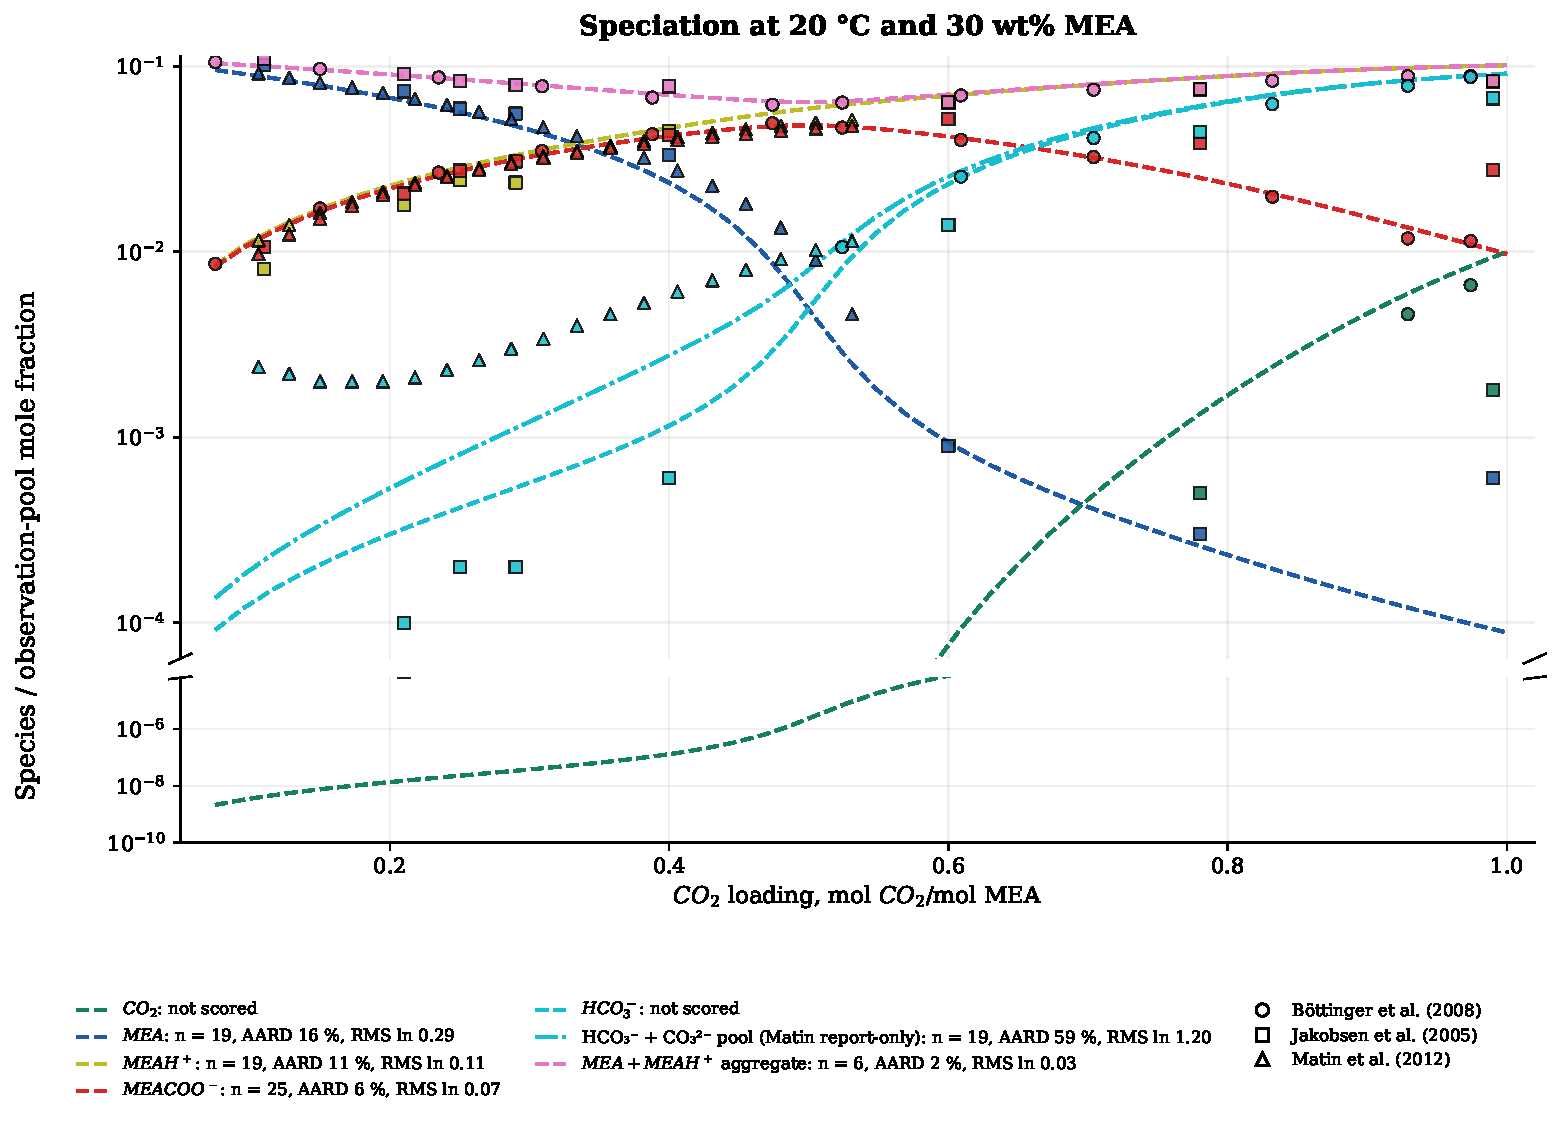
\includegraphics[width=\textwidth]{figures/speciation/output/speciation-diagnostic-replay.pdf}

\small\textbf{Figure 1.} Current smooth-grid diagnostic for the full
nine-species liquid-equilibrium replay at \SI{20}{\celsius} and 30 wt\% MEA.
Symbols show
all positive retained B\"ottinger, Jakobsen, and Matin values for the displayed
series; symbol shape identifies source and color identifies species. The broken
logarithmic axis expands
the $5.6248\times10^{-5}$--0.1134 principal-species region and compresses the
$10^{-10}$--$5.6248\times10^{-5}$ range. Dashed lines connect direct Engine
evaluations of the selected bundle through loading 1.0.
\end{center}

\clearpage
These states are homogeneous reactive-liquid solves, not ideal-reaction or
postprocessed SciPy curves. Each state couples the five reaction constraints
to ePC-SAFT chemical potentials for all nine species at fixed temperature and
pressure. A 2026-09-01 disposable timing check on this machine, excluding
process startup and model construction, measured 0.935 s/state for a warm
five-state second pass with the retained wheel. The same five feeds took
2.260 s/state with a disposable wheel built from Engine main after only the
required provider-to-EOS request-schema renames. This is a route-specific
diagnostic, not a general Engine benchmark: recent GREPE and regression
speedups do not establish a speedup for this homogeneous-liquid owner.
\section{Carbon-dioxide pressure replay}
\label{sec:pressure-replay}

Figure 2 shows all 161 active-v1 30 wt\% MEA pressure observations from
Aronu, Hilliard, Idris, Jou, Mamun, and Xu at 40--\SI{120}{\celsius}. The
selected replay evaluates all 161 states. Its full-data log$_{10}$ RMSE is
0.3317. Lines interpolate the 161 evaluated selected-bundle observation
states; no additional smooth-grid Engine campaign was required, and every
experimental point remains shown.

\begin{center}
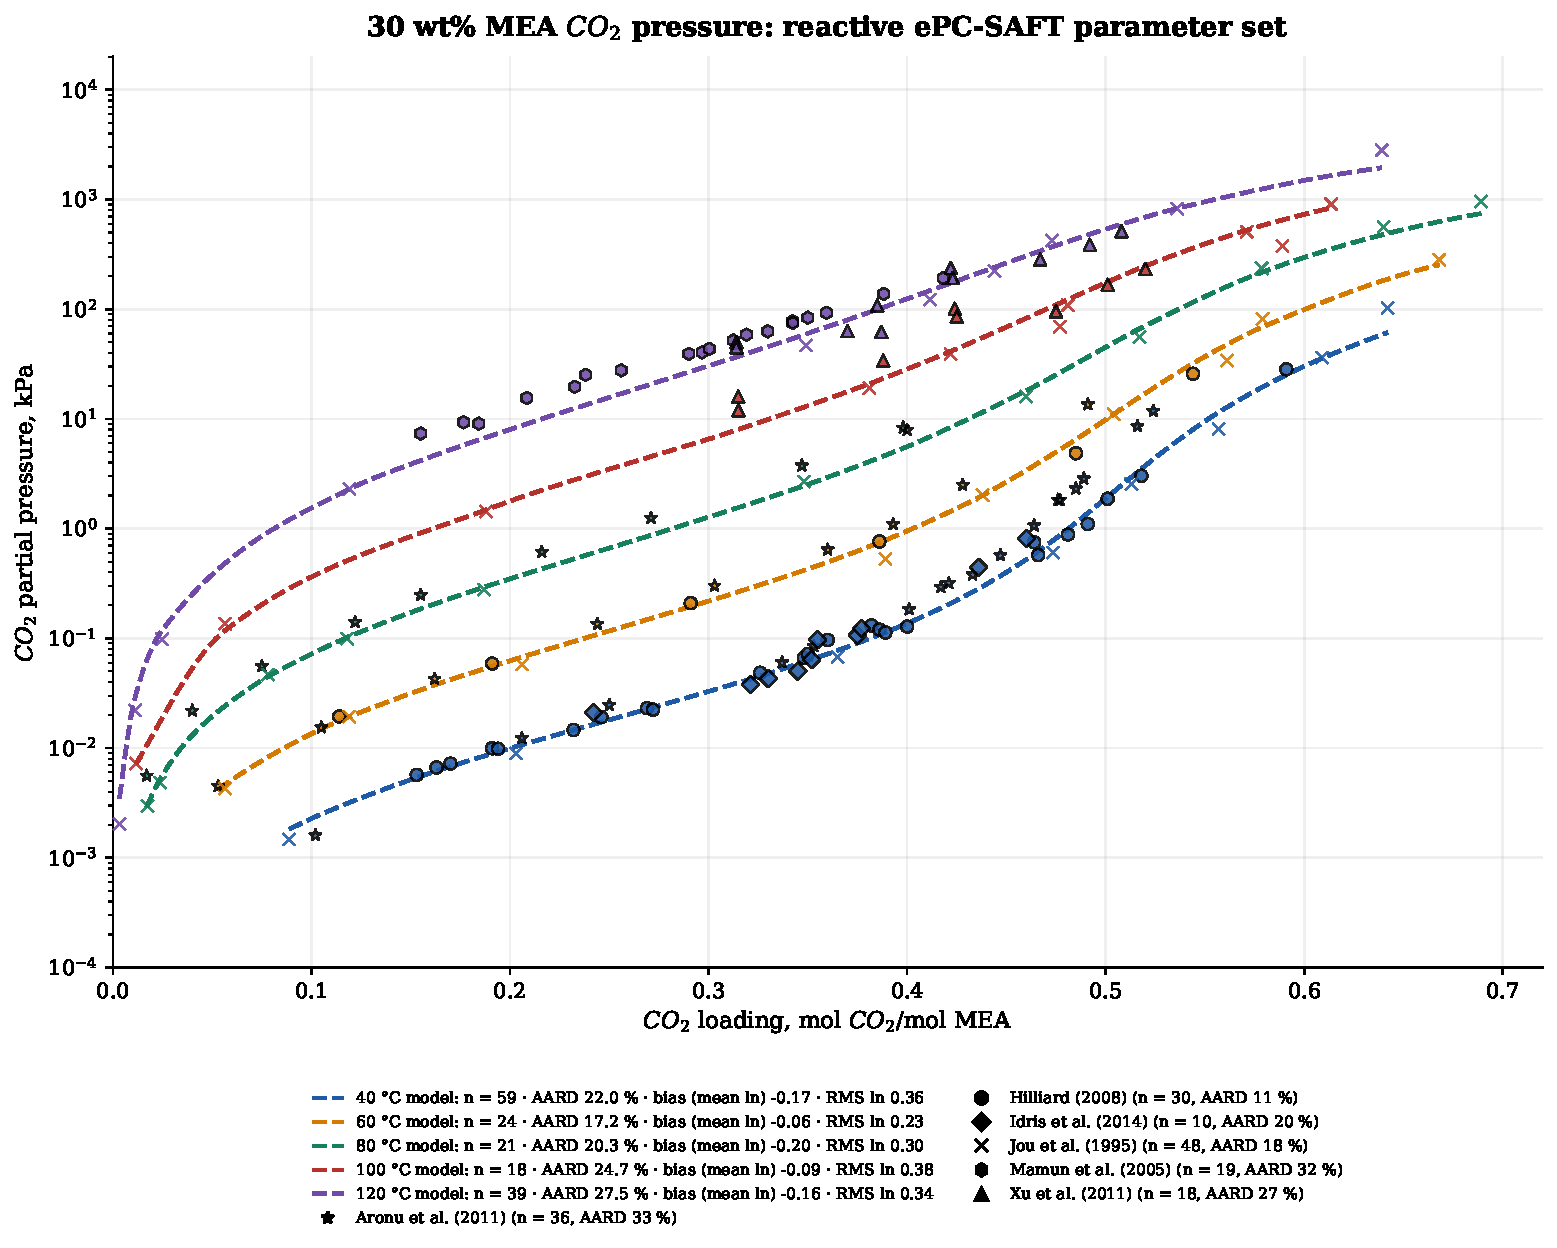
\includegraphics[width=\textwidth]{figures/pressure/output/pressure-diagnostic-replay.pdf}

\small\textbf{Figure 2.} Carbon-dioxide partial pressure for 30 wt\% MEA.
Colors identify temperature, symbols identify experimental source, and lines
are shape-preserving log-response interpolations of newly calculated
active-bundle states within each evaluated loading range; every retained
observation and corresponding model state is included.
\end{center}

The 41 pressure non-evaluations reported by the earlier independent replay
were branch-selection failures, not missing thermodynamic solutions. That
replay rebuilt every row from its source start and discarded the nearest
certified liquid state. In a representative \SI{120}{\celsius} failure, the
inner reactive liquid passed its balance, reaction, pressure, KKT, and local
stability checks, while the outer bubble iteration alternated between about
272 and 739 kPa until its iteration limit. Projecting a certified neighboring
loading or temperature state onto the target balances places the same fixed
parameter problem on the continuous liquid branch. The deterministic replay
now tries that nearest certified branch, retains the original independent
start as a fallback, and uses a neighboring-temperature certified branch only
when needed. It recovers all 41 rows without changing parameters, tolerances,
or iteration limits.

\subsection{Current-bundle fit and coverage statistics}

These are replay/agreement statistics for the exact bundle in
Tables~1--4. Log residuals are
$\log_{10}(y_{\mathrm{model}}/y_{\mathrm{obs}})$; the RMSE factor is
$10^{\mathrm{RMSE}_{\log_{10}}}$. Native pressure errors are in kPa and
native speciation errors are mole fractions.

\begin{center}
\small
\begin{tabular}{@{}lrrrrrr@{}}
\toprule
Family & Coverage & log RMSE & RMSE factor & MAPE (\%) & MAE & Native RMSE \\
\midrule
Pressure & 161/161 & 0.3317 & 2.146 & 55.75 & 48.1848 & 195.5063 \\
Speciation targets & 125/131 & 0.3702 & 2.345 & 23.26 & 0.005180 & 0.008568 \\
\bottomrule
\end{tabular}
\end{center}

Pressure performance and, especially, evaluability vary strongly by
temperature:

\begin{center}
\small
\begin{tabular}{@{}rrrrrr@{}}
\toprule
$T$ (\si{\celsius}) & Coverage & log RMSE & RMSE factor & MAPE (\%) & Median APE (\%) \\
\midrule
40  & 59/59 & 0.2698 & 1.861 & 66.71 & 63.85 \\
60  & 24/24 & 0.2507 & 1.781 & 41.02 & 38.67 \\
80  & 21/21 & 0.4069 & 2.552 & 49.55 & 58.10 \\
100 & 18/18 & 0.3422 & 2.199 & 46.56 & 48.38 \\
120 & 39/39 & 0.4027 & 2.527 & 55.83 & 58.43 \\
\bottomrule
\end{tabular}
\end{center}

The principal measured-species breakdown shows that bicarbonate, not the
amine/carbamate coordinates, dominates the speciation log score:

\begin{center}
\small
\begin{tabular}{@{}lrrrr@{}}
\toprule
Target & Coverage & log RMSE & RMSE factor & MAPE (\%) \\
\midrule
MEA & 18/19 & 0.0582 & 1.143 & 9.70 \\
\ce{MEAH+} & 18/19 & 0.0943 & 1.243 & 23.17 \\
MEA + \ce{MEAH+} & 24/25 & 0.0598 & 1.148 & 9.11 \\
\ce{MEACOO-} & 42/44 & 0.4901 & 3.091 & 14.65 \\
\ce{HCO3-} & 23/24 & 0.5412 & 3.477 & 64.42 \\
\bottomrule
\end{tabular}
\end{center}

The complete machine-readable handoff is retained in the results directory:
\begin{itemize}
\item row-level observed/predicted values: \path{current-best-fit-residuals.csv};
\item grouped overall, temperature, source, species, and temperature--source
statistics: \path{current-best-fit-statistics.csv};
\item failed coordinates and diagnostics: \path{figure-calculation-failures.csv}.
\end{itemize}
The bundle can be used for absorption-column calculations. All 161 retained
pressure observations evaluate, including all 39 at \SI{120}{\celsius}.
Two observed speciation states and three optional smooth-grid states remain
non-evaluable and are explicit in the failure table.

\section{What pressure constrains and what remains unresolved}
\label{sec:pressure-identifiability}

At phase equilibrium the molecular carbon-dioxide fugacities satisfy
\begin{equation}
f_{\ce{CO2}}^{V}=f_{\ce{CO2}}^{L}.
\label{eq:co2-phase-equilibrium}
\end{equation}
An activity/Henry representation writes the same comparison schematically as
\begin{equation}
y_{\ce{CO2}}\phi_{\ce{CO2}}^{V}P
=x_{\ce{CO2}}\gamma_{\ce{CO2}}^{L}H_{\ce{CO2}}.
\label{eq:co2-pressure-constraint}
\end{equation}
\textbf{inference:} pressure observations therefore constrain the liquid
molecular-\ce{CO2} chemical potential together with loading, material balances,
and the reaction network. They are valuable indirect speciation evidence, but
they do not separately identify free $x_{\ce{CO2}}$, liquid nonideality,
reaction constants, association, binary interactions, dielectric terms, or
solvation factors. Direct species observations and pressure observations are
combined because they constrain different projections of the same equilibrium
state; pressure is not a substitute for direct speciation.

\textbf{verified:} the retained replay does not assume an ideal vapor. Its
state packet declares a neutral incipient-vapor phase and reads
\texttt{phase.partial\_pressure} from the pinned ePC-SAFT equilibrium result.
By contrast, the current public IDAES column property files declare an ideal
liquid/Henry-law MEA solvent and an ideal vapor; they are not the modified-eNRTL
model from a separate literature study. The public solvent file retains the
three apparent neutral components \ce{CO2}, MEA, and \ce{H2O} plus the three
ionic species \ce{MEAH+}, \ce{MEACOO-}, and \ce{HCO3-}
\href{https://github.com/IDAES/idaes-pse/blob/main/idaes/models_extra/column_models/properties/MEA_solvent.py}{[official IDAES solvent file]};
the vapor file explicitly selects the ideal equation of state
\href{https://github.com/IDAES/idaes-pse/blob/main/idaes/models_extra/column_models/properties/MEA_vapor.py}{[official IDAES vapor file]}.

\subsection{Reduced-chemistry diagnostic}

The six-species reduction retains \ce{CO2}, MEA, \ce{H2O}, \ce{MEAH+},
\ce{MEACOO-}, and \ce{HCO3-}. To isolate species-set structure without
importing IDAES empirical equilibrium constants, derive its two net constants
from the current five-reaction basis:
\begin{align}
K_{\mathrm{carbamate}} &= \frac{K_2}{K_4K_5}, &
\ce{CO2 + 2MEA <=> MEACOO- + MEAH+},\\
K_{\mathrm{bicarbonate}} &= \frac{K_2}{K_5}, &
\ce{CO2 + MEA + H2O <=> HCO3- + MEAH+}.
\end{align}
The first relation is the exact R2$-$R4$-$R5 projection already recorded in
MEA Issue \#72. This makes the comparison a reaction-space projection of the
same model rather than a change of both chemistry and equilibrium constants.

\textbf{verified:} across the 44 retained nine-species calculations, the
largest mole fractions are $1.0307\times10^{-2}$ for \ce{HCO3-},
$1.1687\times10^{-4}$ for \ce{CO3^2-}, $3.3641\times10^{-6}$ for \ce{OH-},
and $8.9480\times10^{-12}$ for \ce{H3O+}. The largest omitted net-charge
contribution $(2x_{\ce{CO3^2-}}+x_{\ce{OH-}}-x_{\ce{H3O+}})/x_{\ce{MEAH+}}$
is 0.01949 at B\"ottinger state 030. These values are calculated directly
from \path{figures/speciation/output/speciation-model.csv}.

The complete matched comparison is retained under
\path{../enrtl_six_species_ideal_comparison/}; its Quarto source and rendered
PDF are the detailed calculation record. In its ideal-liquid lane, all 232
unique canonical coordinates and 464 model rows converged with a maximum
equation residual of $1.9895\times10^{-13}$. The largest difference among the
six shared species was $6.5100\times10^{-3}$ mol per mol initial MEA, and
carbonate dominated the omitted inventory. In its fixed-$T,P$ Engine/SciPy
lane at \SI{100}{\kilo\pascal}, the carbonate amounts at 293.15, 313.15, and
323.15 K were $2.99\times10^{-4}$, $1.56\times10^{-4}$, and
$1.10\times10^{-4}$ mol per mol initial MEA; the largest shared-species changes
were approximately $2.9\times10^{-4}$ mol per mol initial MEA. That lane is a
liquid-composition calculation, not a bubble-pressure calculation.

\textbf{verified structural result:} when the six- and nine-species states are
both projected to the same conserved apparent totals, their neutral apparent
pressure inputs agree to $1.321165\times10^{-14}$. The neutral
\texttt{flashTQ} route converged for only 1 of 161 pressure observations and
predicted \SI{2038.38}{\kilo\pascal} for an observed
\SI{0.00202}{\kilo\pascal}. A neutral apparent flash therefore cannot reveal
the internal reaction or ionic parameters; the pressure calculation must keep
the reactive species allocation coupled to the EOS.

The companion sensitivity survey evaluated 143 parameter identities grouped
into 113 continuous directions with 128 Latin-hypercube samples, of which 123
were usable. Its strongest recurring directions were R5 $a_K$, R4 $b_K$, the
water segment-diameter temperature terms, \ce{MEAH+} dispersion and ionic
terms, and selected \ce{CO2}--water, carbonate--water, MEA--\ce{MEAH+},
\ce{MEAH+}--water, carbamate--hydronium, and bicarbonate--\ce{CO2} binary
interactions. Those numerical ranks belong to parameter packet
\nolinkurl{0e7c5ac63c078be9d32c15f316ecdb2b0de67de6f495358ab5955450f0271c6a}
and Engine-wheel hash
\nolinkurl{05cca73463b9b44dcb3a77dfd239b767ec63aafce7d18b85b2a66b80773847a5};
the separate fixed-$T,P$ lane used packet
\nolinkurl{12e380a27eb615e25bae580f8c1ec852020879917b08fa16a5821ae76311550d}.
Neither is the active bundle in Tables~1--3, so the
ranking must be replayed with the active parameter file before its numerical
ordering is used in the manuscript.

\textbf{inference:} the three omitted trace ions have small direct abundance
over this replay, which makes a six-species ablation useful as a cheap
conditioning test. It does not prove that they are dispensable: the
$z_i^2$ weighting gives carbonate four times the per-mole ionic-strength
contribution of a monovalent ion, and the omitted species preserve carbonate,
autoprotolysis, pH, charge, and extrapolation structure. Removing them also
removes weakly identified ionic parameters, so an apparent fit improvement may
come from reduced flexibility rather than better physics.

\begin{center}
\small
\begin{tabularx}{\textwidth}{@{}p{0.27\textwidth}YY@{}}
\toprule
Retained finding & Present use & Remaining action \\
\midrule
Exact R2--R4--R5 and R2--R5 projection & Methods description for a controlled six-species ablation & None for the algebra; cite the retained reaction table. \\
Ideal and fixed-$T,P$ species comparison & Evidence that carbonate is the dominant omitted species and that the reduction is not simple deletion & Repeat the coupled bubble calculation with the active bundle before using pressure-error conclusions. \\
Neutral apparent-pressure invariance & Methods/diagnostic explanation of why total absorbed carbon cannot be passed directly to a neutral \ce{CO2} flash & Keep as a route-rejection result; do not present the 1/161 flash as a model fit. \\
Packet-specific sensitivity survey & Prioritizes the first active-bundle sensitivity directions & Replay the same screen with the active parameter mapping and wheel before reporting ranks or intervals. \\
\bottomrule
\end{tabularx}
\end{center}

\section{Interpretation}

The R4--\ce{CO2} update reduces pressure error while preserving complete observed-
speciation coverage, but the residual changes sign with temperature and
all 39 pressure states at \SI{120}{\celsius} now evaluate. The remaining
temperature-dependent mismatch is therefore a model residual rather than a
coverage artifact; it does not justify opening R1--R3, R5, or the ion block as
compensating coordinates.

The Class 1 $k_{\ce{CO2},\mathrm{MEA}}=0$ uses the uncorrected combining rule;
it does not assert an absence of physical interaction. The bounded screen shows
that one constant correction is too weak and too temperature uneven to explain
the observations, so this coordinate is not a present refinement priority.
Likewise, loaded-MEA
pressure alone cannot identify $f_{\mathrm{solv},\ce{CO2}}$ or
$f_{\mathrm{solv},\mathrm{MEA}}$ because those working assumptions are confounded with
cross association, dielectric response, reaction, and other physical
interactions.

Historical diagnostics remain outside the bundle:
\begin{itemize}
\item legacy $k_{\ce{CO2},\mathrm{MEA}}=-0.1957268589$;
\item alternate \ce{MEAH+} $\sigma=2.753332853$ and \ce{MEACOO-}
  $\sigma=3.017079292$; and
\item trace-only bicarbonate Born-diameter movement toward
  \SI{6.80294}{\angstrom}, with \ce{CO3^2-} left near
  \SI{2.99744}{\angstrom}.
\end{itemize}
These values identify sensitivity or lineage; none is adopted. The
trace-carbonate result does not establish independent identifiability.

\subsection{Source-derived regression rules to preserve}
\label{sec:regression-rules}

The following rules are retained because they change how a future MEA fit must
be designed. They are methodological constraints from the ePC-SAFT lineage,
not additional fitted results.

\begin{description}
\item[Select the formulation before estimating its parameters.] B\"ulow and
Ascani show that the Born expression, composition-dependent permittivity, and
their complete composition derivatives change electrolyte activities and
phase partitioning; Ascani's solvent-mass and combined rules can reverse a
failed salting-out prediction without introducing ion--solvent corrections
\cite[Secs.~3.2--4]{Bulow2020}\cite[pp.~1310--1313]{Ascani2021}. Therefore a
parameter vector fitted under one Born/permittivity formulation cannot be
treated as an unchanged control under another. The fixed-parameter structural
screen in Section~\ref{sec:permittivity-comparison} must precede any refit.

\item[Keep parameter blocks with the model choices that generated them.]
Pabsch et al. explicitly retain the 2B water model because the inherited ion
parameters were estimated with that water parameterization; changing the water
association scheme would require refitting the ion block
\cite[p.~5770]{Pabsch2020}. The same restriction applies to the reciprocal
induced \ce{CO2}--\ce{H2O} topology: a $k_{ij}$ obtained with non-induced
\ce{CO2} is not interchangeable with the present induced-association value.

Baygi and Pahlavanzadeh additionally show why pure-fluid agreement cannot
select an MEA association topology: their 2B, 3B, and 4C MEA fits gave similar
pure saturation behavior but different aqueous binary VLE and excess-enthalpy
behavior \cite[pp.~789, 795--799]{Baygi2015}. Their nonionic PC-SAFT study
selected 3B MEA with 4C water, but that result does not authorize replacing the
present 2B/2B reactive ePC-SAFT block. It instead requires any future topology
comparison to refit the complete coupled block and judge binary and caloric
observables, not pure density and vapor pressure alone.

\item[Assign each coordinate an identifying observable.] The literature's
useful hierarchy is: neutral pure-component parameters from density and vapor
pressure; neutral binary and cross-association corrections from binary VLE;
ionic short-range parameters and ion--water corrections from aqueous density,
osmotic coefficients, or MIACs; $d_i^{\mathrm{Born}}$ from ion-specific
infinite-dilution solvation evidence; and solvent $f_{\mathrm{solv}}$ from
finite-concentration MIACs. Figiel then performs one joint iteration and finds
only minimal movement \cite[p.~9411]{Figiel2025}. Reactive MEA pressure may
test the assembled bundle, but it should not be the sole datum identifying
every block.

\item[Keep reaction constants, activities, and standard states together.]
Uyan et al. solve chemical and phase equilibrium with ePC-SAFT activities and
show that replacing species activities by mole fractions worsens the species
distribution \cite[pp.~96--98]{Uyan2015}. Therefore R1--R5 coefficients cannot
be transplanted, refitted, or compared independently of their concentration
scale, reference states, and activity-coefficient convention. Pressure is an
indirect reaction constraint; admitted speciation and caloric observations are
needed to prevent an EOS parameter from compensating for an inconsistent
reaction basis.

\item[Use simpler electrolyte subsystems to resolve reactive-mixture gaps.]
Uyan et al. set the unsupported water--\ce{MDEAH+} correction to zero when no
pseudo-binary data were available \cite[p.~95]{Uyan2015}. Wangler et al. later
found water--\ce{HCO3-} and water--\ce{MDEAH+} influential, estimated them from
aqueous \ce{NaHCO3} and protonated-MDEA osmotic-coefficient data, and then
predicted the reactive \ce{CO2}--water--MDEA VLE without fitting that ternary
pressure data \cite[pp.~19--24]{Wangler2018}. The MEA analogue is to seek
aqueous bicarbonate and protonated-MEA salt activity or osmotic evidence before
using reactive pressure to adjust the corresponding binary terms.

\item[Do not call calibration rows predictions.] Uyan and Wangler reserve
``prediction'' for reactive ternary gas-solubility results after parameters
were obtained from pure fluids and binary or pseudo-binary subsystems
\cite{Uyan2015,Wangler2018}. Any future use of MEA pressure or speciation rows
in the objective must label those rows calibration and report performance on
held-out temperatures and sources separately.

\item[Compare model error with experimental disagreement.] Pabsch et al.
screen conflicting \ce{CO2}-solubility sources before fitting and compare the
model AARD with the inter-source ARSD; similar magnitudes indicate that the
experimental record, rather than only the model, limits apparent accuracy
\cite[pp.~5771--5775]{Pabsch2020}. The MEA campaign should retain source-wise
residuals and duplication structure rather than assigning equal confidence to
every digitized row.

\item[Treat single-ion solvation values as convention-dependent anchors.]
B\"ulow et al. note that individual-ion hydration Gibbs energies are not
directly measurable and are assembled through extra-thermodynamic conventions
\cite[Sec.~3.2]{Bulow2020}. They are useful for ranking and anchoring Born
diameters, but agreement with one tabulation is not independent proof of a
unique physical radius. Salt-level MIAC, transfer, density, and osmotic data
remain necessary checks.

\item[Bind every result to the exact corrected parameter packet.] The B\"ulow
corrigendum reports a parameter error in the published MIAC calculations and
replaces Figs.~6--7 while leaving the qualitative conclusions unchanged
\cite{Bulow2021b}. This is direct precedent for retaining source corrections,
unrounded parameter files, Engine identity, and hashes; a figure or rounded
table alone is not a reproducible parameter authority.

\item[Use caloric behavior as a reaction-model check.] Wangler et al. use
absorption enthalpy as a downstream prediction and connect its quality to the
reaction equilibria and the temperature and composition dependence of species
activities \cite[pp.~24--26]{Wangler2018}. After pressure and speciation are
stable, retained MEA absorption-enthalpy data provide an independent test of
R1--R5 that pressure-only refinement cannot supply.
\end{description}

\subsubsection{Absorption-enthalpy observations and required calculation}
\label{sec:calorimetry-plan}

The repository already contains the observations needed for a paired-state
calorimetry study; no data import from the eNRTL fitting repository is needed.
The canonical table \path{MEA_heat_of_absorption_observations.csv} is retained
under \path{data/reference/MEA/observations/calorimetry/}. Its exact SHA-256 is
recorded in the calculation receipt.
The materialized campaign view preserves every source field and adds the
partition, pair group, preceding endpoint, and two required sensitivity labels.

\begin{center}
\small
\begin{tabularx}{\textwidth}{@{}lrrY@{}}
\toprule
Source and temperature & Rows & Role & Use \\
\midrule
Kim--Svendsen 2007, 40 and \SI{80}{\celsius} & 66 & Calibration & Available for a bounded joint pressure--species--enthalpy fit. \\
Kim--Svendsen 2007, \SI{120}{\celsius} & 20 & Temperature holdout & Evaluate after model selection; do not use it to pull the temperature fit. \\
Kim et al. 2014, Table A1-1 & 27 & Model-selection comparison & The earlier eNRTL study inspected these rows, so they are not untouched validation for that candidate. \\
\bottomrule
\end{tabularx}
\end{center}

The Engine now supplies complete reactive total enthalpy on the solved-pressure
bubble-point route. The current bundle was therefore replayed without fitting
against all 113 retained calorimetry observations. All 113 endpoint states and
all 113 finite loading intervals evaluated. The overall RMSE is 23.98, the
mean bias is $-18.57$, and the median absolute error is 19.25
\si{\kilo\joule\per\mole} \ce{CO2}. The calibration partition gives RMSE
20.01, the Kim et al. model-selection comparison gives 16.84, and the
\SI{120}{\celsius} temperature holdout gives 39.30
\si{\kilo\joule\per\mole} \ce{CO2}. The fixed bundle therefore
systematically underpredicts heat release, with the largest disagreement at
the held-out high temperature.

\begin{figure}[H]
\centering
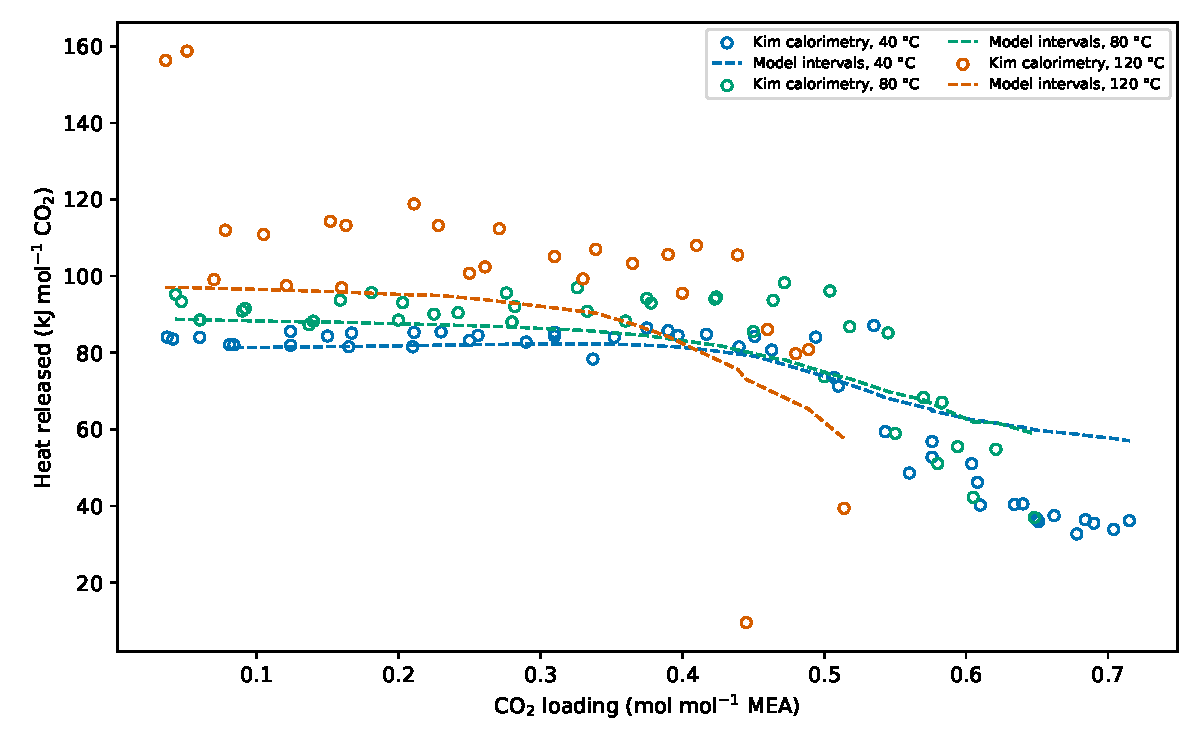
\includegraphics[width=0.92\textwidth]{figures/calorimetry/output/current-selected-direct-enthalpy.pdf}
\caption{Retained calorimetry observations (points) and the current fixed
Tables~1--4 bundle evaluated by direct total reactive enthalpy (continuous
lines). Lines are shape-preserving interpolations of the scored finite-interval
predictions; no calorimetry parameter was fitted.}
\label{fig:current-selected-calorimetry}
\end{figure}

For adjacent loading endpoints $i-1$ and $i$ in one source, temperature,
MEA concentration, and experimental run, the modeled positive heat-release
magnitude must be
\begin{equation}
q_i^{\mathrm{model}}=-\frac{
n_i h_{L,i}-n_{i-1}h_{L,i-1}
-\Delta n_{\ce{CO2},i}h_{\ce{CO2},\mathrm{ig}}(T)}
{\Delta n_{\ce{CO2},i}}.
\label{eq:calorimetry-paired-state}
\end{equation}
Here $n h_L$ is total equilibrium-liquid enthalpy, not residual enthalpy alone;
$h_{\ce{CO2},\mathrm{ig}}$ is incoming ideal-gas carbon-dioxide enthalpy on the
same reference basis; and the leading minus sign converts an exothermic
enthalpy change to the reported positive release magnitude in
\si{\kilo\joule\per\mole} \ce{CO2}. The first modeled endpoint in each
series uses the declared starting-loading assumption
$\alpha_{\ce{CO2}}=0.003$; that assumption and the likely source typo at
\texttt{kim2007\_t40\_r1\_0.041} require separate exclusion or perturbation
checks \cite[Table~1, p.~3]{Kim2007}.

This is a direct finite-dose energy balance, not a pressure-slope estimate.
For each endpoint the same nine-species reactive liquid is solved, and the
Engine combines declared species reference enthalpies with the active ePC-SAFT
residual departure. Reaction heat is not added as a separate empirical
correction: it enters through the equilibrium species amounts on one common
standard-state enthalpy basis.

The caller-owned reference thermochemistry is constructed without calorimetry
fitting. At 313.15, 353.15, and \SI{393.15}{\kelvin}, the Engine evaluates the
source-to-EOS temperature transfer and the typed R1--R5 correlations give
\begin{equation}
\Delta_r h_r^\circ=RT^2\left(\frac{\partial\ln K_{r,\mathrm{EOS}}}
{\partial T}\right),\qquad
\mathbf{h}^\circ=\mathbf{S}^{\mathsf T}
(\mathbf{S}\mathbf{S}^{\mathsf T})^{-1}\boldsymbol{\Delta_r h}^\circ.
\label{eq:reaction-consistent-enthalpy-gauge}
\end{equation}
The second relation chooses a deterministic minimum-norm conserved gauge.
The \SI{393.15}{\kelvin} calorimetry results extrapolate R5 beyond its stated
323.15 K correlation domain, so the large \SI{120}{\celsius} disagreement is
evidence for the next reaction-temperature study rather than a validated
high-temperature R5 prediction.
Quadratic interpolation through the three temperature knots supplies one
reference enthalpy and linear heat-capacity polynomial per species. The same
thermochemistry fingerprint is used at every loading, and the Engine
independently checks $\mathbf{S}\mathbf{h}^\circ=RT^2\partial\ln\mathbf{K}/
\partial T$ before returning an enthalpy.

The retained wheel is built from Engine commit
\nolinkurl{8438ce5f94a547189c91c4ec180a7782d60879d6}. Upstream PRs 199--201 add
reference-consistent total enthalpy, correct the reference-pressure derivative,
and preserve reaction-temperature derivatives through solved-pressure and
incipient-boundary reconstruction. The final replay required 191 solver
attempts: 78 initial starts failed before a certified neighboring-loading or
neighboring-temperature continuation recovered the same state. No tolerance,
iteration limit, parameter, or equation was changed, and no endpoint remains
failed. The earlier high-temperature gaps were initialization-path failures in
the outer bubble-pressure route, not absent thermodynamic solutions.

The present reconstruction assumes zero finite vapor inventory in the
calorimeter and incoming ideal-gas \ce{CO2} with zero residual enthalpy on the
same gauge. Those assumptions are explicit in the retained receipt. The older
Gibbs--Helmholtz diagnostic remains useful as an independent pressure-slope
comparison, but it is no longer the primary calorimetry result. Both methods
show the same negative heat-release bias. The direct result identifies a real
model deficiency, but it does not by itself distinguish reaction temperature
coefficients from missing reference heat-capacity or residual-enthalpy
structure. The next fit should therefore use the smallest supported R1--R5
enthalpy-coordinate subset and judge it simultaneously against pressure,
speciation, and the untouched \SI{120}{\celsius} holdout.

The calorimetry view is retained at
\path{data/input/calorimetry-observation-partition.csv} within this analysis.
Its receipt records 113 rows in nine pair groups, positive loading increments,
the canonical and selected-view hashes, and the two sensitivity requirements.
This prepares the evidence without changing the active parameter mapping.

\subsubsection{Current bundle against those rules}

The current bundle is usable as the best retained working bundle, but it is not
equally mature in every parameter block. ``Meets'' below means that the present
lineage and experiment are appropriate; it does not mean that the numerical
value can never be revised.

\begin{center}
\small
\begin{tabularx}{\textwidth}{@{}p{0.20\textwidth}p{0.14\textwidth}YY@{}}
\toprule
Block & Assessment & Present evidence & Consequence \tabularnewline
\midrule
Model structure & Meets & 2B water and MEA, reciprocal induced
\ce{CO2}--\ce{H2O} association, solvent-only mass-fraction permittivity, and
automatic SSM+DS were evaluated as one declared structure. & Keep automatic
activation fixed while profiling the active Born diameters and neutral
solvation factors together. \tabularnewline
Neutral molecular block & Mostly meets & Water and MEA coordinates retain
literature lineages; $k_{\ce{MEA},\ce{H2O}}$ and
$k_{\ce{CO2},\ce{H2O}}$ were fitted to their binary systems with the active
association choices. & Do not reopen the neutral block broadly. The locally
adjusted $\epsilon_{\ce{CO2}}/k$ must be called a reactive-MEA calibration
coordinate and checked on held-out sources. \tabularnewline
Reaction block & Partial & R1--R5 use a coherent standard-state conversion,
but R4 was adjusted with $\epsilon_{\ce{CO2}}/k$ against reactive pressure and
the older sensitivity survey identified R5 as influential. & Recompute
active-bundle R4/R5 sensitivities and use pressure, species, and direct
absorption enthalpy together; do not infer either reaction solely from
pressure. \tabularnewline
Principal amine ions & Needs stronger anchors & The \ce{MEAH+} and
\ce{MEACOO-} molecular and Born coordinates are local Class~3 fit outputs from
8 states and 22 residuals, with only a small total improvement and two failed
final evaluations. & Seek protonated-MEA salt and carbamate-relevant
electrolyte evidence before another broad reactive-mixture fit. \tabularnewline
Carbonate and trace ions & Partial & Literature molecular rows are retained,
but the \ce{HCO3-}/\ce{CO3^2-} Born diameters have only a paired coarse screen
and the \ce{OH-} diameter is a local inversion. Bicarbonate log-RMSE is 0.6154,
far larger than the other measured species. & Prioritize bicarbonate chemistry,
the carbonate Born radii, and their water interactions in a controlled
active-bundle identifiability screen. \tabularnewline
Binary interaction matrix & Mixed & Literature-zero corrections are fixed,
three nonzero water--trace-ion transfers remain Class~2, and seven zero pairs
were sensitive only in an older packet. & Replay only those named Class~2
directions with the active packet before promoting any $k_{ij}$ to a fit
coordinate. \tabularnewline
\bottomrule
\end{tabularx}

\vspace{8pt}

\begin{tabularx}{\textwidth}{@{}p{0.20\textwidth}p{0.14\textwidth}YY@{}}
\toprule
Evidence lane & Assessment & Present evidence & Consequence \tabularnewline
\midrule
Pressure and numerical coverage & Complete for observations & Pressure
log-RMSE is 0.3317 for 161/161 states, including 39/39 at
\SI{120}{\celsius}. The mean residual is positive at \SI{40}{\celsius} and
negative from 60 through \SI{120}{\celsius}. & Use all observations in later
model comparisons; do not reinterpret the recovered rows as new experimental
evidence. \tabularnewline
Speciation & Mixed & 125/131 positive observed targets evaluate. MEA and
\ce{MEAH+} remain comparatively strong at log-RMSE 0.0582 and 0.0943, while
\ce{MEACOO-} and \ce{HCO3-} are weak at 0.4901 and 0.5412. & Preserve the
free/protonated-amine behavior and target carbamate--bicarbonate coupling
rather than globally refitting every ion.
\tabularnewline
Permittivity and solvation & Conditional & The active bundle uses solvent-only
mass-fraction mixing with automatically activated SSM+DS, but no independent
loaded-MEA static-permittivity data validate the predicted response. & Obtain
that evidence and jointly profile $f_{\mathrm{solv},\mathrm{MEA}}$ with the
uncertain Born diameters. \tabularnewline
Calibration separation & Partial & Source-wise residuals, hashes, and exact
packets are retained, but the selected R4--\ce{CO2} update used the current
reactive observations. & Freeze explicit calibration and held-out source or
temperature partitions before the next parameter optimization. \tabularnewline
Absorption enthalpy & Complete fixed-bundle replay & The Engine returns
reference-consistent total reactive enthalpy, and all 113 retained intervals
evaluate. Overall RMSE is 23.98 and the \SI{120}{\celsius} holdout RMSE is
39.30 \si{\kilo\joule\per\mole} \ce{CO2}. & Use the systematic negative bias
to constrain a small reaction-temperature coordinate set while preserving the
current pressure and speciation performance. \tabularnewline
\bottomrule
\end{tabularx}
\end{center}

\textbf{Current diagnosis.} The neutral and association foundation is the
strongest part of the bundle, and free/protonated-amine speciation is described
well. The immediate scientific weaknesses are bicarbonate and carbamate,
followed by insufficiently anchored ionic/Born coordinates. The former
high-temperature bubble-pressure coverage weakness has been removed for the
retained pressure observations by preserving certified loading and temperature
continuation states. Three optional smooth
speciation-grid points remain non-evaluable. Solver coverage and scientific
fit must remain separate: a recovered solve is not evidence for a different
parameter value, and a converged residual is not evidence that the ionic block
is identified.

\subsection{Full-domain permittivity selection}
\label{sec:permittivity-comparison}

This fixed-parameter structure study asks how the current solvent-only
mass-fraction rule with automatically selected SSM+DS compares with the
previous original-Born baseline and other source-consistent structures in its
combined description of reactive MEA pressure, speciation, dielectric
response, and physical branch identity. It changes no
reaction, molecular, ionic, association, binary, vapor, tolerance, or
initialization input. Reciprocal induced \ce{CO2}--\ce{H2O} association and
the unique Born diameters in Table~2 remain active in every calculation. No
parameter was fitted.

\subsubsection{Equations, pools, units, and derivatives}

Let $N=\{\ce{H2O},\ce{MEA},\ce{CO2}\}$, $I$ be the six charged species in
Table~2, $x_N=\sum_{j\in N}x_j$, and
$w_j^N=x_jM_j/\sum_{k\in N}x_kM_k$. Rule A intentionally uses the explicit
solvent pool $N_A=\{\ce{H2O},\ce{MEA}\}$. Rules B--E include molecular
\ce{CO2} explicitly. No rule silently removes or renormalizes another
component. The screened bulk relative-permittivity rules
are
\begin{align}
\epsilon_r^A &= \sum_{j\in N_A}w_j^{N_A}\epsilon_{r,j},
&\text{solvent-only mass-fraction mixing},\label{eq:eps-a}\\
\epsilon_r^B &= \sum_{j\in N\cup I}x_j\epsilon_{r,j},
&\text{all-component mole-fraction mixing},\label{eq:eps-b}\\
\epsilon_r^C &= \frac{\sum_{j\in N\cup I}x_jM_j\epsilon_{r,j}}
{\sum_{j\in N\cup I}x_jM_j},
&\text{all-component mass-fraction mixing},\label{eq:eps-c}\\
\epsilon_r^D &= x_N\sum_{j\in N}w_j^N\epsilon_{r,j}
 +\sum_{i\in I}x_i\epsilon_{r,i},
&\text{combined solvent-mass/ion-mole mixing},\label{eq:eps-d}\\
\epsilon_r^E &= \frac{\epsilon_{r,N}^{\mathrm{salt\text{-}free}}}
{1+7.01x_I},\qquad x_I=\sum_{i\in I}x_i,
&\text{nonlinear ionic suppression}.\label{eq:eps-e}
\end{align}
Rules B--D use $\epsilon_{r,i}=8$ for every ion. The pure-component inputs
are the retained water correlation, $\epsilon_{r,\mathrm{MEA}}=32$, and the
Schick transfer
$\epsilon_{r,\ce{CO2}}(T)=1.4122-0.0036(T-293\,\mathrm{K})$
\cite[Table~2]{Schick2023}. Equations~\ref{eq:eps-a}--\ref{eq:eps-d} use the
three linear mixing forms and salt-free-solvent definition reported by Ascani
and Held \cite[Eqns.~11--13]{Ascani2021}; Rule A retains only the normalized
salt-free-solvent average within Equation~13. Equation~\ref{eq:eps-e} is the
nonlinear empirical electrolyte-suppression rule fitted at \SI{298.15}{K}
\cite[Eqns.~11--12]{Figiel2025}. Relative permittivity, $f_{\mathrm{solv}}$,
$c_{\mathrm{shell}}$, and $c_{\mathrm{dielectric}}$ are dimensionless;
$d_i^{\mathrm{Born}}$ is stored in \si{\angstrom} and converted to metres.
The exact source locators are B\"ulow's original-Born Eq.~2 and
composition-derivative Eqs.~3--5, with the linear dielectric discussion around
Eq.~7; the B\"ulow corrigendum's correction to the input used in Figs.~6--7;
Ascani's Born Eq.~10 and mixing Eqs.~11--13; and Figiel's SSM+DS Eqs.~6--10,
nonlinear dielectric Eqs.~11--12, and Supporting Information Table~1,
Table~S2, and Figs.~S1--S6. The corrigendum reports that the corrected figures
do not change B\"ulow's conclusions. The full receipt records separate
SHA-256 identities for the B\"ulow article, its corrigendum, the Ascani
article, the Figiel article, and the Figiel Supporting Information rather
than treating any pair as one source.

Rule A applies the normalized salt-free-solvent average to water and MEA.
Dissolved molecular \ce{CO2} and all ions therefore have zero direct weight
in this rule. This descriptive name identifies the equation and component
pool without attaching a system-specific parameter-set name to it.

For rules with temperature-dependent pure-component values, the exact Engine
automatic derivatives follow the declared algebra. For example,
$\partial\epsilon_r^B/\partial x_i=\epsilon_{r,i}$ and, if
$\epsilon_r^C=N_C/M_C$,
$\partial\epsilon_r^C/\partial x_i=M_i(\epsilon_{r,i}M_C-N_C)/M_C^2$.
The corresponding temperature derivatives sum the pure-component
$\partial\epsilon_{r,j}/\partial T$ terms; all five rules have
$\partial\epsilon_r/\partial\rho=0$. Rules D and E use exact quotient and
chain derivatives rather than frozen-composition approximations.

The original Born residual is
\begin{equation}
\frac{a^{\mathrm{Born}}}{RT}=-\frac{e^2}{4\pi\epsilon_0k_BT}
\sum_{i\in I}x_i z_i^2\frac{1-1/\epsilon_r}{d_i^{\mathrm{Born}}}.
\label{eq:born-original}
\end{equation}
The corrected Engine SSM+DS form first defines
\begin{equation}
d_i^{\mathrm{out}}=d_i^{\mathrm{Born}}
\left[1+c_{\mathrm{shell}}\frac{f_{\mathrm{mix}}-1}{|z_i|}\right],
\qquad f_{\mathrm{mix}}=
\frac{\sum_{j\in S}x_jf_{\mathrm{solv},j}}{\sum_{j\in S}x_j},
\end{equation}
and replaces the radial factor in Equation~\ref{eq:born-original} by
\begin{equation}
\frac{1-1/\epsilon_r}{d_i^{\mathrm{out}}}
+c_{\mathrm{dielectric}}\left(1-\frac{1}{\epsilon_{r,i}^{\mathrm{local}}}\right)
\left(\frac{1}{d_i^{\mathrm{Born}}}-\frac{1}{d_i^{\mathrm{out}}}\right),
\qquad \epsilon_{r,i}^{\mathrm{local}}=8.
\label{eq:ssmds-corrected}
\end{equation}
The active parameter contract does not store these switches. If at least one
ion declares a positive unique $d_i^{\mathrm{Born}}$ and at least one neutral
component declares $f_{\mathrm{solv}}\ne1$, the Engine derives
$c_{\mathrm{shell}}=c_{\mathrm{dielectric}}=1$. Otherwise it derives zero for
both. A declared ionic $d_i^{\mathrm{Born}}=0$ is not a zero physical radius:
it is materialized as the same resolved ion diameter used by Debye--H\"uckel,
$d_i^{\mathrm{DH}}=0.88\sigma_i$, which recovers the original-Born convention
reported by B\"ulow et al. Explicit switch values remain accepted only for
exact replay of older immutable packets.
$S$ is the explicit solvation pool: every component with a declared
$f_{\mathrm{solv},j}$. The primary Figiel calculations include all nine
species in $S$; the coupled \ce{CO2}-exclusion calculation omits molecular
\ce{CO2} from both $S$ and the salt-free neutral-permittivity pool. Thus
``CO2 excluded'' means both that \ce{CO2} is not treated as a solvent-like
contributor to $f_{\mathrm{mix}}$ and that it does not contribute to the
salt-free neutral dielectric average; \ce{CO2} remains a full reacting EOS
component. No
composition is silently renormalized outside the denominators shown above.
Equation~\ref{eq:ssmds-corrected} is the Engine's corrected nested radial
charging expression, not the misprinted ordering in Figiel's printed Eq.~7.
The Engine differentiates Equations~\ref{eq:born-original}--
\ref{eq:ssmds-corrected} with respect to temperature, density, composition,
and active parameters.

The six fixed MEA-study Born diameters are
\SI{3.5332}{\angstrom} (\ce{MEAH+}), \SI{3.5411}{\angstrom}
(\ce{MEACOO-}), \SI{3.0000}{\angstrom} (\ce{HCO3-}),
\SI{3.0000}{\angstrom} (\ce{CO3^2-}), \SI{1.2180}{\angstrom}
(\ce{H3O+}), and \SI{3.0811}{\angstrom} (\ce{OH-}). They were held fixed in
every structure comparison. Figiel et al. instead fitted aqueous
infinite-dilution solvation data for \ce{H+}, \ce{Li+}, \ce{Na+}, \ce{K+},
\ce{VO2+}, \ce{V^3+}, \ce{Cl-}, \ce{Br-}, \ce{I-}, and \ce{SO4^2-}; their
Table~2 diameters are respectively 1.218, 2.784, 3.445, 4.150, 2.930, 2.940,
4.100, 4.480, 4.985, and \SI{4.953}{\angstrom} \cite{Figiel2025}. Only the
\ce{H3O+}/\ce{H+} value in the present bundle is an exact overlap. Figiel
does not supply diameters for \ce{MEAH+}, \ce{MEACOO-}, \ce{HCO3-},
\ce{CO3^2-}, or \ce{OH-}; substituting Na, halide, or sulfate values for those
chemically different ions would not be source-consistent. A later diameter
regression must therefore use ion solvation or other ion-specific evidence,
not arbitrary cross-ion substitution.

The ``ion-specific'' $\alpha_i$ screen also needs qualification. Zuber
et al.'s Table~2 directly gives 9.55 for \ce{H+} and 13.96 for \ce{OH-}, which
map exactly to the present \ce{H3O+} and \ce{OH-} records
\cite{Zuber2014}. The present values 2.60 for \ce{MEAH+}, 7.01 for
\ce{MEACOO-}, and 7.89 for each carbonate species are project-declared
analogs or fallbacks; Zuber did not fit those MEA-system ions. Consequently
I--SSM+DS is an analog/fallback sensitivity, not a complete
literature-matched ion-specific package.

The retained derivative audit independently perturbed one interior
composition direction for Rules B and C. Analytic and centered finite-
difference derivatives agree to relative errors of
$2.21\times10^{-11}$ and $1.95\times10^{-12}$, respectively; the exact
inputs and step are retained in
\path{results/born-permittivity-study/component-permittivity-derivative-check.json}.

\subsubsection{Automatic activation and unique-diameter sensitivity}

The current screen starts from the selected bundle in Tables~1--4: solvent-only
mass-fraction permittivity, automatically activated SSM+DS, and R5
$a_K=2597.91$ K. It evaluates the complete parameter bundle against the same
12 retained sparse states for every perturbation. Each unique ion Born
diameter was moved by $\pm10\%$; $f_{\mathrm{solv},\mathrm{MEA}}$ was tested
at 1.0, 1.4, 1.5, and 1.6; and the $f_{\mathrm{solv},\mathrm{MEA}}=1.5$
case was crossed with each diameter movement. Pairwise statistics use only
the exact positive targets shared by the perturbed and selected bundles, while
failed states remain in the state table.

The selected bundle evaluates all 12 states. Its sparse pressure and species
log$_{10}$ RMSE are 0.4300 and 0.1246. Changing the \ce{H3O+} or \ce{OH-}
diameter is numerically flat at this resolution. Individually, a 10\% larger
\ce{HCO3-} diameter gives the clearest ion-radius direction, although two
states fail and its pairwise improvements are only 0.0191 for pressure and
0.0033 for species. The MEA solvation-factor series is much more informative:
1.4, 1.5, and 1.6 all reduce both errors on all shared targets; 1.6 gives the
smallest species RMSE and 1.4 the smallest pressure RMSE in that one-coordinate
series.

The strongest fully evaluated joint direction is
$f_{\mathrm{solv},\mathrm{MEA}}=1.5$ with a 10\% larger \ce{HCO3-} Born
diameter. It retains all 12 states and changes pressure RMSE from 0.4300 to
0.3795 and species RMSE from 0.1246 to 0.0771. This is a screening direction,
not a replacement parameter bundle; it is promoted below to the complete
205-state replay before any parameter is changed.

\begin{figure}[H]
\centering
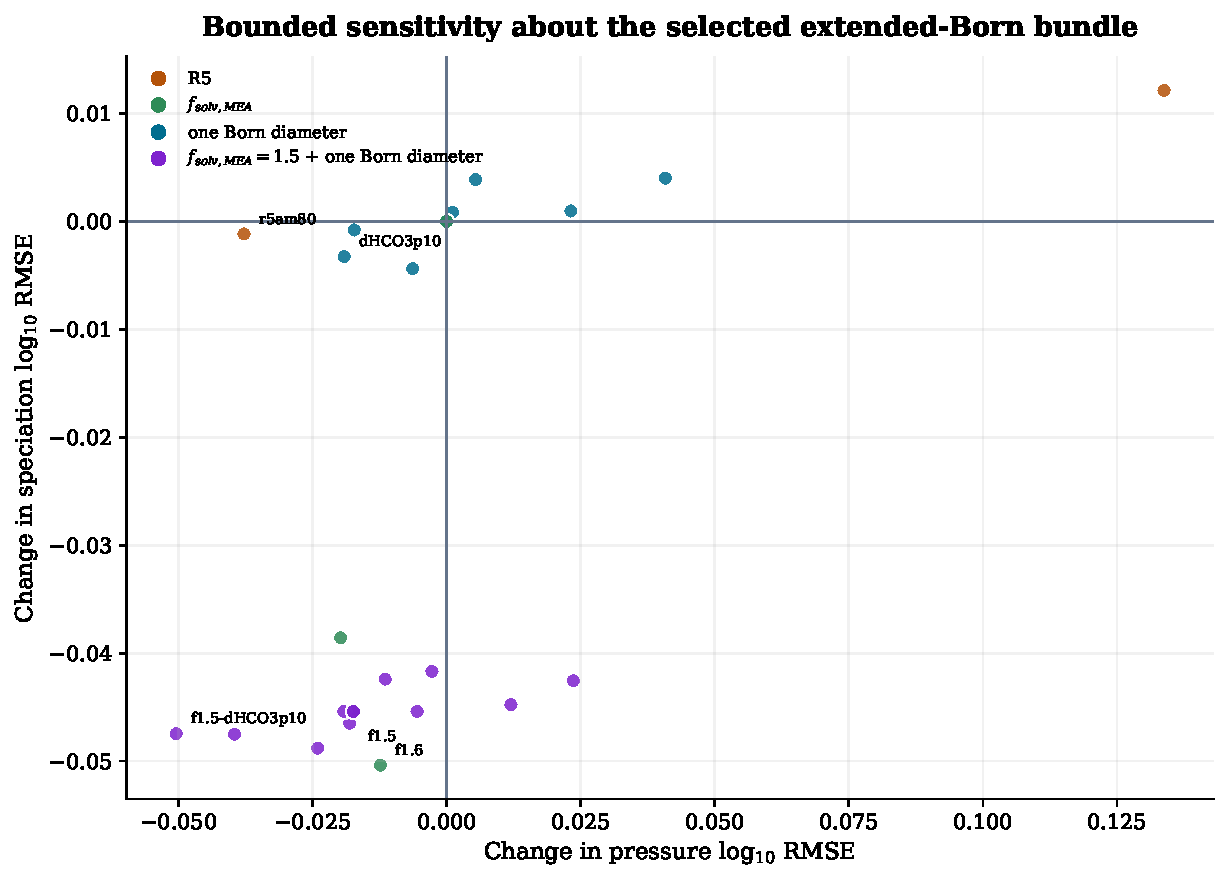
\includegraphics[width=0.88\textwidth]{figures/born_permittivity/output/selected-bundle-joint-sensitivity.pdf}
\caption{Pairwise common-target sensitivity about the selected extended-Born
and R5-adjusted bundle. Negative changes improve agreement. The lower-left
quadrant improves pressure and speciation simultaneously.}
\label{fig:selected-bundle-joint-sensitivity}
\end{figure}

Exact row-level values, failures, pairwise comparisons, and the immutable
receipt are retained under
\path{results/born-permittivity-study/selected-bundle-joint-sensitivity-*}.

The complete replay changes the decision. On the 108 positive pressure
targets evaluated by both bundles, the joint candidate reduces pressure
log$_{10}$ RMSE from 0.3424 to 0.2842 and median factor from 1.8364 to 1.5477.
On all 131 common species targets, however, it increases speciation RMSE from
0.2373 to 0.2600. Numerical coverage changes only from 164 to 165 of 205
states. The direction is therefore useful for a later joint pressure,
speciation, and calorimetry fit, but it does not replace the selected balanced
bundle in Tables~1--4.

\begin{figure}[H]
\centering
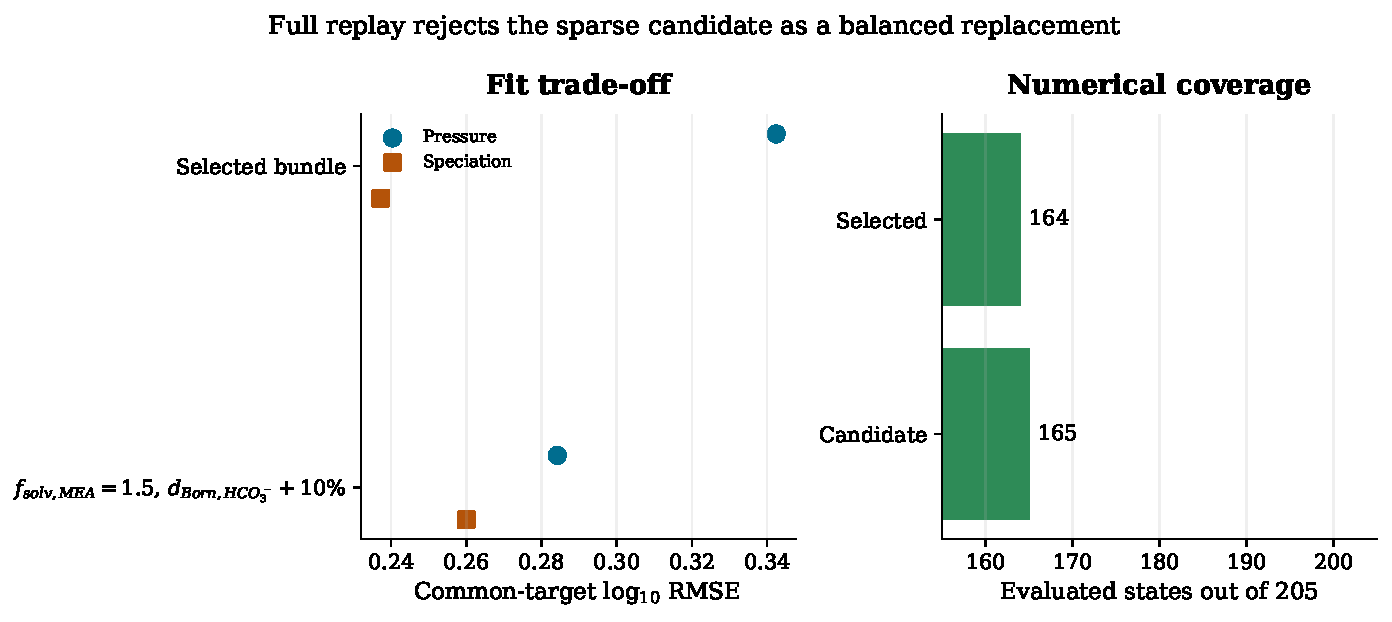
\includegraphics[width=0.92\textwidth]{figures/born_permittivity/output/selected-bundle-full-candidate-comparison.pdf}
\caption{Complete 205-state comparison of the selected bundle and the best
sparse Born/solvation direction. The pressure gain is real on identical
targets, but it comes with worse full speciation.}
\label{fig:selected-bundle-full-candidate}
\end{figure}

\subsubsection{Sparse structure screen}

The first screen used 12 retained states: low, middle, and high loading at the
two best-covered pressure temperatures (40 and \SI{60}{\celsius}) and the two
best-covered speciation temperatures (20 and \SI{40}{\celsius}). All five
permittivity rules were crossed with original Born and SSM+DS. The following table reports
evaluated attempts and positive-target log$_{10}$ RMSE. The attempt count is
a solver diagnostic, not an acceptance cutoff or scientific ranking
coordinate.

\begin{center}
\small
\begin{tabular}{@{}lrrrrr@{}}
\toprule
Variant & States & $\epsilon_r$ range & $p_{\ce{CO2}}$ RMSE & Pressure factor & Species RMSE \\
\midrule
A original & 12/12 & 57.13--79.29 & 0.2704 & 1.4008 & 0.0551 \\
A SSM+DS & 10/12 & 57.13--79.08 & 0.4910 & 2.7414 & 0.1358 \\
B original & 12/12 & 57.98--74.39 & 0.5017 & 2.6384 & 0.0728 \\
B SSM+DS & 9/12 & 57.57--74.28 & 0.5742 & 4.3025 & 0.1451 \\
C original & 12/12 & 43.03--63.78 & 0.9231 & 8.2675 & 0.0761 \\
C SSM+DS & 12/12 & 42.55--63.73 & 0.4020 & 2.4929 & 0.1317 \\
D original & 12/12 & 56.51--70.73 & 0.4645 & 2.8418 & 0.0514 \\
D SSM+DS & 11/12 & 56.50--69.66 & 0.5251 & 3.8518 & 0.1193 \\
E original & 11/12 & 34.63--60.22 & 1.3375 & 26.3051 & 0.0299 \\
E SSM+DS & 12/12 & 32.68--60.03 & 0.4669 & 2.2065 & 0.0960 \\
\bottomrule
\end{tabular}
\end{center}

SSM+DS does not improve every dielectric rule. It increases both errors for
A, B, and D; it reduces the pressure RMSE by 0.5211 for C
while increasing the species RMSE by 0.0555; and it reduces the E-rule pressure
RMSE by 0.8705, but increases the species
RMSE by 0.0660. Thus the apparent rescue of the Figiel package is primarily
the corrected SSM+DS radial work, whereas the large baseline differences among
A--E arise from the permittivity rule itself. This interaction rules out a
single independent ``Born correction'' effect.

Because E--SSM+DS completed the sparse screen, the permitted follow-up tested
universal 7.01 against Zuber-derived analog/fallback $\alpha_i$, and
$f_{\mathrm{solv},\mathrm{MEA}}=1.0,1.4,1.5,1.6$. The 1.5 sparse case lost two
states despite its smaller pressure RMSE; 1.4 and 1.6 completed all 12. An
exact post-solve pool crossover at the 12 converged 1.6 compositions found
$x_{\ce{CO2}}\leq0.002918$, $|\Delta\epsilon_r|\leq0.2663$ (0.813\%), and
$|\Delta f_{\mathrm{mix}}|\leq0.001249$ when \ce{CO2} was excluded. That
algebraic result was used only as a cheap preliminary screen. The promoted
comparison below then re-solved every state with molecular \ce{CO2} removed
from both pools so pressure, speciation, phase identity, and convergence were
tested in the coupled system.

\subsubsection{Complete retained-state comparison}

Each promoted configuration is one complete nine-species parameter bundle.
Every configuration attempted the same 161 active pressure observations from
313.15 to 393.15 K and the same 44 speciation states from 293.15 to 353.15 K;
only the stated permittivity or Born coordinates differ among rows. This gives
1,640 configuration--state attempts in total. The Engine wheel used for that
historical screen preserved the known-state result to numerical precision.
Its parity timing was
measured on the immediate predecessor candidate at Engine commit
\nolinkurl{355d950}; the complete comparison used the final
\nolinkurl{d8e02e4} immutable study wheel, which adds explicit neutral-pool
exclusion, its tested derivatives, and preservation of final partial evidence
at the unchanged bubble-iteration limit. The same solver path, tolerances,
and starts were used. Those timings are retained only as historical
reproducibility metadata; the reaction-synchronized scientific comparison
below uses the current wheel and a three-CPU execution cap.

The Engine's fixed-pressure density anchor was measured separately at
\texttt{vle\_obs\_0140}. Eight single-threaded repetitions reduced median
\texttt{Mixture.state} time from 58.98 to 14.76 ms and density iterations from
30 to 1 (4.00 times), with zero pressure or density difference. The present
reactive equilibrium callable owns its density closure and does not expose
this anchor, so the measurement did not alter the formulation campaign.

The separate 319-row cross-validation inventory remains non-executable: all
319 rows lack a residual scale and immutable data packet, and the 198
speciation rows also lack a fixed-pressure definition. The 123-state immutable
packet used here is already executable and is not evidence that those broader
admission decisions are resolved.

\setcounter{figure}{2}
\begin{figure}[H]
\centering
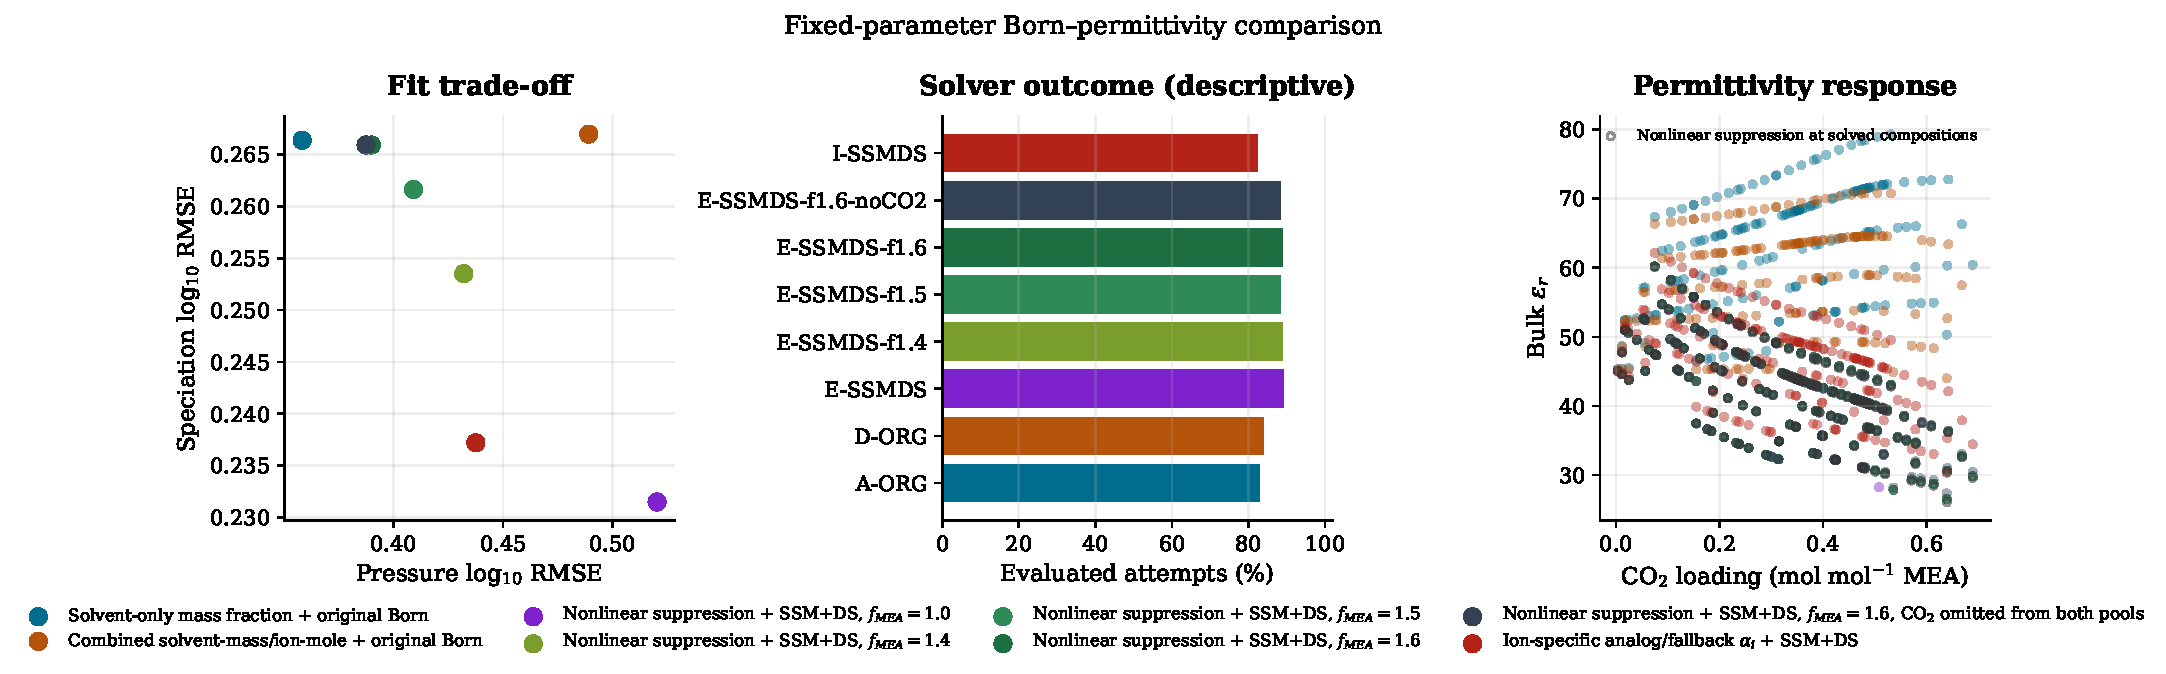
\includegraphics[width=\textwidth]{figures/born_permittivity/output/born-permittivity-overview.pdf}
\caption{Fixed-parameter trade-off, descriptive evaluated-attempt fraction, and bulk relative
permittivity for every promoted configuration. The open circles apply the
nonlinear ionic-suppression equation to solvent-only-mass-fraction/original-
Born solved compositions; they are a crossover, not
independent loaded-MEA dielectric observations. Attempt fraction is not used
to rank formulations.}
\label{fig:born-permittivity-overview}
\end{figure}

\begin{center}
\small
\begin{tabularx}{\textwidth}{@{}Yrrrrrr@{}}
\toprule
Variant & $N_p/161$ & $p_{\ce{CO2}}$ log RMSE & Factor & Bias & $N_x/44$ & $x$ log RMSE \\
\midrule
A: solvent-only mass fraction + original Born & 126/161 & \textbf{0.3583} & \textbf{1.9577} & 0.0956 & 44/44 & 0.2664 \\
D: combined mixing + original Born & 128/161 & 0.4892 & 2.5954 & 0.2763 & 44/44 & 0.2670 \\
E: nonlinear suppression + SSM+DS, $f_{\mathrm{MEA}}=1.0$ & 139/161 & 0.5204 & 2.7461 & 0.2372 & 44/44 & \textbf{0.2315} \\
E: nonlinear suppression + SSM+DS, $f_{\mathrm{MEA}}=1.4$ & 138/161 & 0.4321 & 2.2891 & 0.2177 & 44/44 & 0.2535 \\
E: nonlinear suppression + SSM+DS, $f_{\mathrm{MEA}}=1.5$ & 138/161 & 0.4092 & 2.1997 & 0.2114 & 43/44 & 0.2616 \\
E: nonlinear suppression + SSM+DS, $f_{\mathrm{MEA}}=1.6$ & 138/161 & 0.3899 & 2.1264 & 0.2074 & 44/44 & 0.2659 \\
E: nonlinear suppression + SSM+DS, $f_{\mathrm{MEA}}=1.6$, no \ce{CO2} & 137/161 & 0.3875 & 2.1090 & 0.2066 & 44/44 & 0.2659 \\
Ion-specific suppression + SSM+DS & 125/161 & 0.4376 & 2.3821 & \textbf{0.0710} & 44/44 & 0.2372 \\
\bottomrule
\end{tabularx}
\end{center}

The table reports each complete bundle against both observation families.
Its full-data metrics use every successful calculation for that bundle, so
different numerical failures can change the rows entering a metric. A second,
common-observation calculation therefore compares all eight bundles on the
exact positive pressure-observation intersection ($n=102$) and, separately,
on the exact positive speciation-observation intersection ($n=129$). The two
intersections differ because pressure and liquid composition are different
measured quantities, not because a different parameter bundle was used.
On these common observations, solvent-only mass fraction with original Born
has the smallest pressure log RMSE (0.3544; median factor 1.8607), while
nonlinear suppression with SSM+DS and $f_{\mathrm{MEA}}=1.0$ has the smallest
speciation log RMSE (0.2333). No row is selected from only one observation
family. The complete common-observation table is retained in
\path{results/born-permittivity-study/full-common-row-statistics.csv}.

\paragraph{Current reaction-synchronized result.}
The preceding eight-configuration screen is retained as model-structure
history, but its observation requests embedded an older R4 correlation and
therefore do not describe the present parameter bundle. The current comparison
rebuilds every request from the displayed R1--R5 correlations and uses Engine
commit \nolinkurl{8438ce5f94a547189c91c4ec180a7782d60879d6}. Each complete
nine-species configuration was evaluated against the same 205 states. Metrics
below use the exact intersection of 100 positive pressure targets and 123
positive speciation targets evaluated by all four configurations; coverage is
reported separately, so no configuration benefits from silently dropping a
difficult observation.

\begin{center}
\small
\begin{tabularx}{\textwidth}{@{}Yrrrrrr@{}}
\toprule
Complete configuration & States & $p_{\ce{CO2}}$ RMSE & Factor & Bias & Species RMSE & Species factor \\
\midrule
Solvent-only mixing, original Born & 171/205 & \textbf{0.3386} & \textbf{1.8652} & 0.0982 & 0.2734 & 1.0713 \\
Solvent-only mixing, SSM+DS, literature R5 & 161/205 & 0.4930 & 2.4745 & $-0.4073$ & 0.2676 & 1.2281 \\
Selected: solvent-only mixing, SSM+DS, R5 $a_K=2597.91$ K & 164/205 & 0.3456 & 1.8672 & $-0.1532$ & 0.2442 & 1.1466 \\
Nonlinear suppression, SSM+DS, R5 $a_K+80$ K & \textbf{174/205} & 0.4417 & 2.3122 & \textbf{$-0.0199$} & \textbf{0.2440} & \textbf{1.0961} \\
\bottomrule
\end{tabularx}
\end{center}

\begin{figure}[H]
\centering
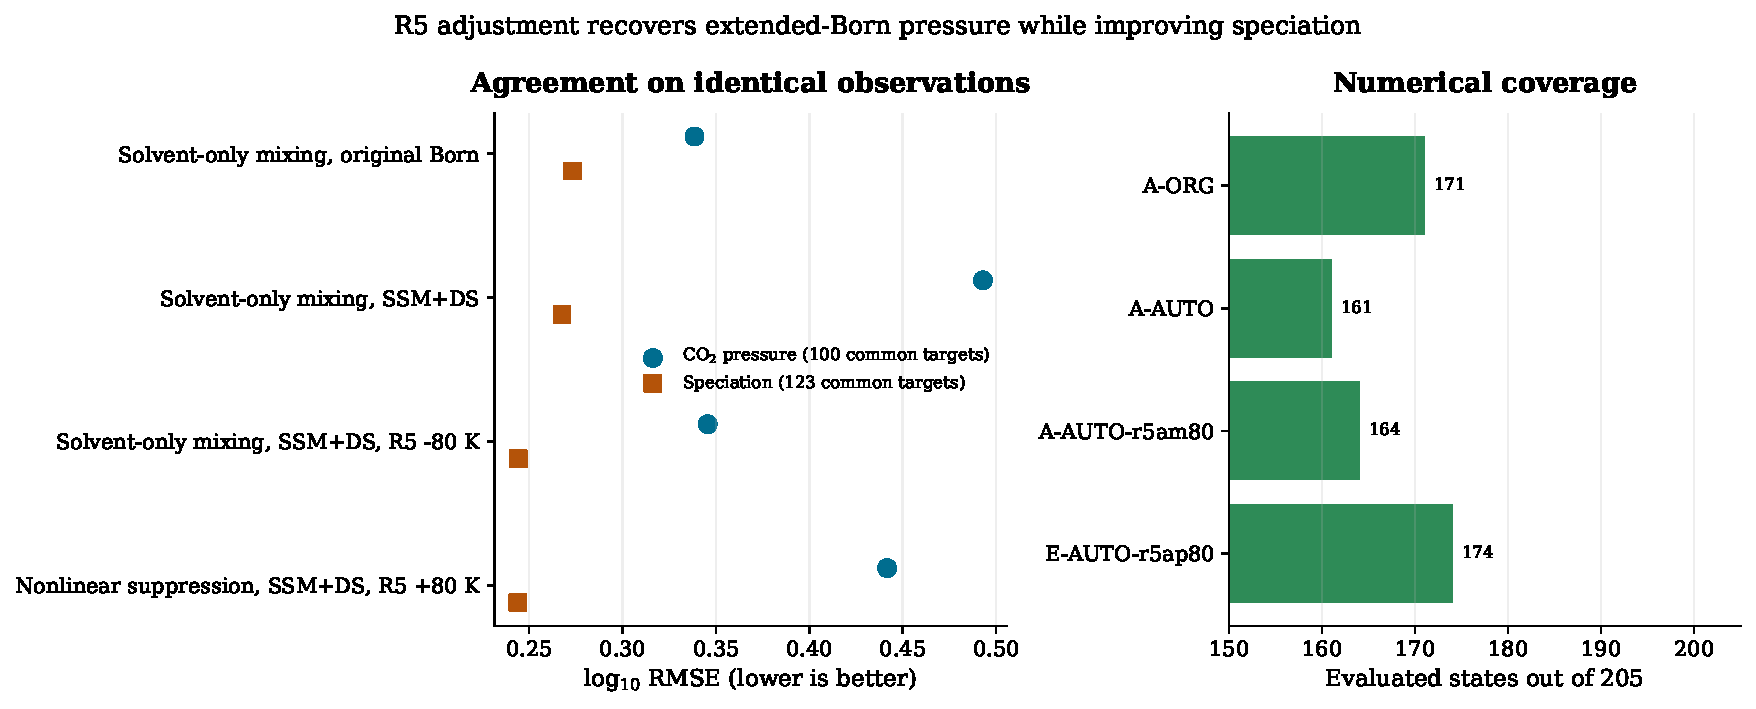
\includegraphics[width=\textwidth]{figures/born_permittivity/output/current-fast-born-reaction-comparison.pdf}
\caption{Current reaction-synchronized comparison. Pressure and speciation
log$_{10}$ RMSE use observations evaluated by all four configurations
($n_p=100$, $n_x=123$); the right panel reports all successful states out of
205 attempts. Lower RMSE is better.}
\label{fig:current-born-reaction-comparison}
\end{figure}

No single row wins every quantity. Original Born gives the smallest common-row
pressure RMSE. Nonlinear suppression with SSM+DS and R5 $a_K+80$ K gives the
largest evaluated-state count, nearly zero mean pressure bias, and the smallest
species RMSE, but its pressure scatter remains larger. The best tested balance
and the selected active bundle is solvent-only mixing with SSM+DS and
R5 $a_K=2597.91$ K: relative to original
Born, its pressure RMSE is only 0.0070 larger while its species RMSE is 0.0292
smaller. Relative to the unadjusted SSM+DS bundle, it reduces pressure RMSE by
0.1474 and species RMSE by 0.0233.

The opposite useful R5 directions under the two permittivity rules are the
central result. R5 is not an independent correction that can be transferred
unchanged between Born/permittivity formulations: reaction speciation changes
liquid composition and CO2 activity, which changes bubble pressure, while the
electrostatic formulation changes the activities entering R5. The fixed-R5
comparison therefore diagnosed coupling rather than proving that original Born
is intrinsically superior. A defensible next fit must estimate R5 together with
the uncertain ion Born diameters and neutral solvation factors under one chosen
permittivity formulation, using both pressure and speciation residuals.

The four current calculations preserve 34, 44, 41, and 31 failed states,
respectively. The nonlinear-suppression row improves coverage but does not
eliminate the high-temperature pressure failures. Those states remain solver
evidence and must be recovered before the formulation comparison is considered
complete. Exact values are retained in the Born--permittivity study results
directory: \texttt{current-fast-common-comparison.csv}, with row-level states
and targets in the \texttt{corrected-reaction-full} and
\texttt{figiel-r5-positive-full} result families.

Figure~\ref{fig:born-permittivity-residuals} shows that every configuration
shares the same principal pressure pattern: negative low-loading residuals,
positive middle-loading residuals, and a temperature-dependent high-loading
return. The speciation statistic is dominated by underprediction of
\ce{HCO3-}; the other reported quantities cluster near zero residual. The
grouped heat map makes the temperature, source, and species dependence
explicit.

\begin{figure}[H]
\centering
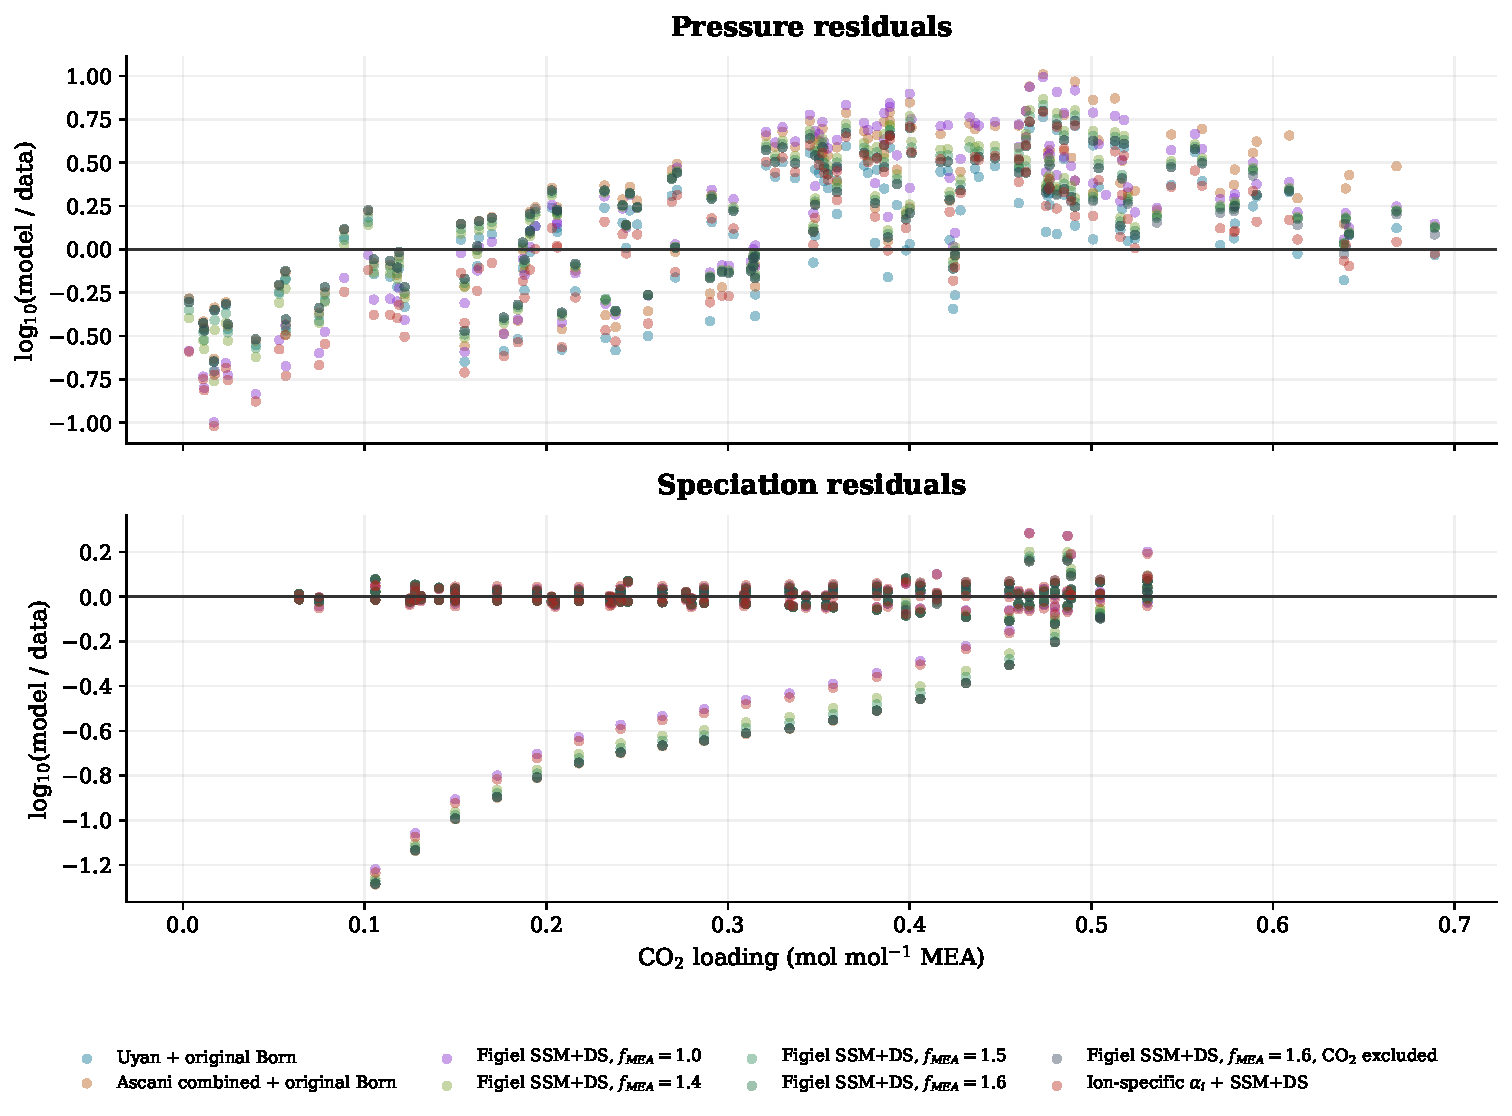
\includegraphics[width=0.94\textwidth]{figures/born_permittivity/output/born-permittivity-residuals.pdf}
\caption{All positive observed--predicted pressure and speciation residuals.
Every point is a direct retained Engine evaluation; no curve or failed state
has been interpolated.}
\label{fig:born-permittivity-residuals}
\end{figure}

\begin{figure}[H]
\centering
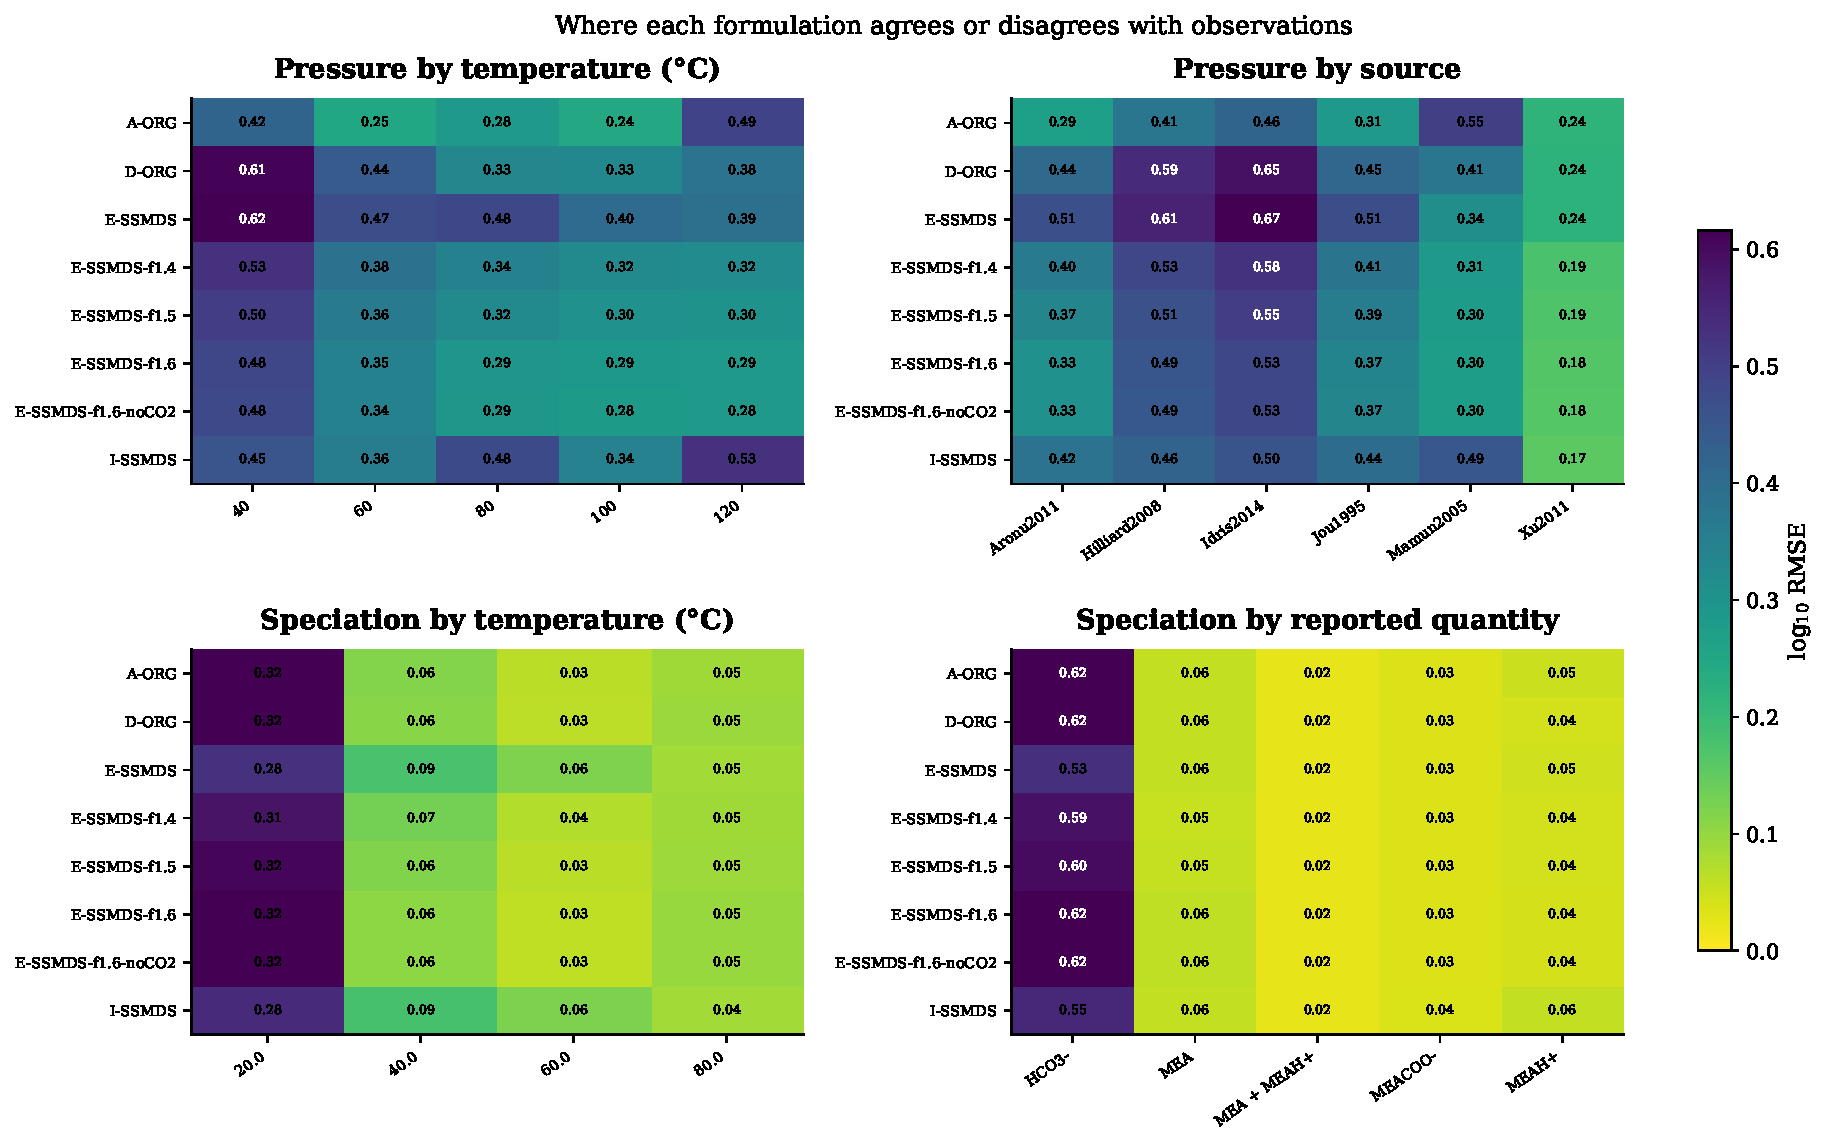
\includegraphics[width=\textwidth]{figures/born_permittivity/output/born-permittivity-grouped-residuals.pdf}
\caption{Log$_{10}$ RMSE grouped by pressure temperature and source, and by
speciation temperature and reported quantity. Missing groups remain missing
rather than being imputed.}
\label{fig:born-permittivity-grouped}
\end{figure}

Every evaluated liquid state is on an accepted liquid mechanical branch, and
every incipient vapor is on its accepted vapor branch. Maximum absolute charge
closure is below $2.4\times10^{-17}$, material closure below
$2.8\times10^{-13}$, reaction-affinity closure below
$1.3\times10^{-11}$, and relative pressure closure below
$6.4\times10^{-10}$. Figure~\ref{fig:born-permittivity-diagnostics} retains
the density range, closure values, and all 220 non-evaluable attempts. Of
those, 181 reach the existing bubble-pressure Newton iteration limit, 38
produce a finite phase candidate that does not pass the complete equilibrium
certificate, and one stops in the inner IPOPT solve. The complete row-by-row
table records source, temperature, loading, continuation and start
availability, and stopping point. The former label ``request-policy
validation'' was a reporting defect: an empty policy record hid the native
``bubble Newton iteration limit reached'' result. Engine commit
\nolinkurl{d8e02e4} preserves the last partial state and policy so that the
actual failure is now retained. These are execution boundaries, not evidence
that a physical formulation is false.

\begin{center}
\small
\begin{tabular}{@{}llrrr@{}}
\toprule
Source & Temperature (\si{\celsius}) & Bubble iteration & Certificate & Inner solve \\
\midrule
Aronu 2011 & 40, 60, 80 & 0 & 14 & 0 \\
B\"ottinger 2008 & 20 & 0 & 1 & 0 \\
Hilliard 2008 & 40 & 0 & 13 & 1 \\
Idris 2014 & 40 & 0 & 1 & 0 \\
Jou 1995 & 40, 60, 80, 120 & 42 & 5 & 0 \\
Mamun 2005 & 120 & 70 & 1 & 0 \\
Xu 2011 & 100, 120 & 69 & 3 & 0 \\
\midrule
Total & & 181 & 38 & 1 \\
\bottomrule
\end{tabular}
\end{center}

These counts are formulation--state attempts over 60 distinct observations.
All failures had a continuation value. Of the 181 bubble-iteration stops, 165 used one
pressure start without a liquid start and 16 also had a liquid start. Of the
39 later stops, 38 used one pressure start and one certification failure had
no pressure start. The exact loading and per-variant record remains in
\path{results/born-permittivity-study/full-failure-characterization.csv}.

All 38 certificate failures compiled, completed the inner solve, passed the
EOS-domain check, and returned a locally evaluable candidate, but no candidate
passed the full closure and local-stability certificate. Thirty-seven are
reported as numerical-convergence failures; one E--SSM+DS,
$f_{\mathrm{MEA}}=1.5$ attempt at \SI{20}{\celsius} is a physical-rejection
classification with material closure 0.0243, reaction-affinity closure 1.893,
KKT closure 0.0125, and failed local stability. The same observation evaluates
under the other seven configurations. The single IPOPT failure likewise
occurs for one configuration of a row evaluated by most alternatives. These
facts make all 39 candidate/inner-solve failures branch-and-initialization
robustness evidence, not proof that the observed state or formulation is
physically impossible.

The 181 bubble failures are concentrated at high temperature: 182 of all 220
non-evaluable configuration--state attempts occur at \SI{120}{\celsius}, with
the remainder at 20, 40, 60, 80, and \SI{100}{\celsius}. Increasing the outer
iteration cap from 18 to 60 and sweeping pressure starts from 10 kPa to 5 MPa
did not recover the representative \SI{120}{\celsius} row; iterates alternated
between gas-like and dense-liquid roots. The required Engine experiment is
therefore a branch-aware coupled pressure KKT formulation, not looser
tolerances or more iterations. Every one of these 181 rows is retained as an
acceptance case: the structural comparison must be rerun after that solver
change, and no present attempt count is used to rank formulations.

\begin{figure}[H]
\centering
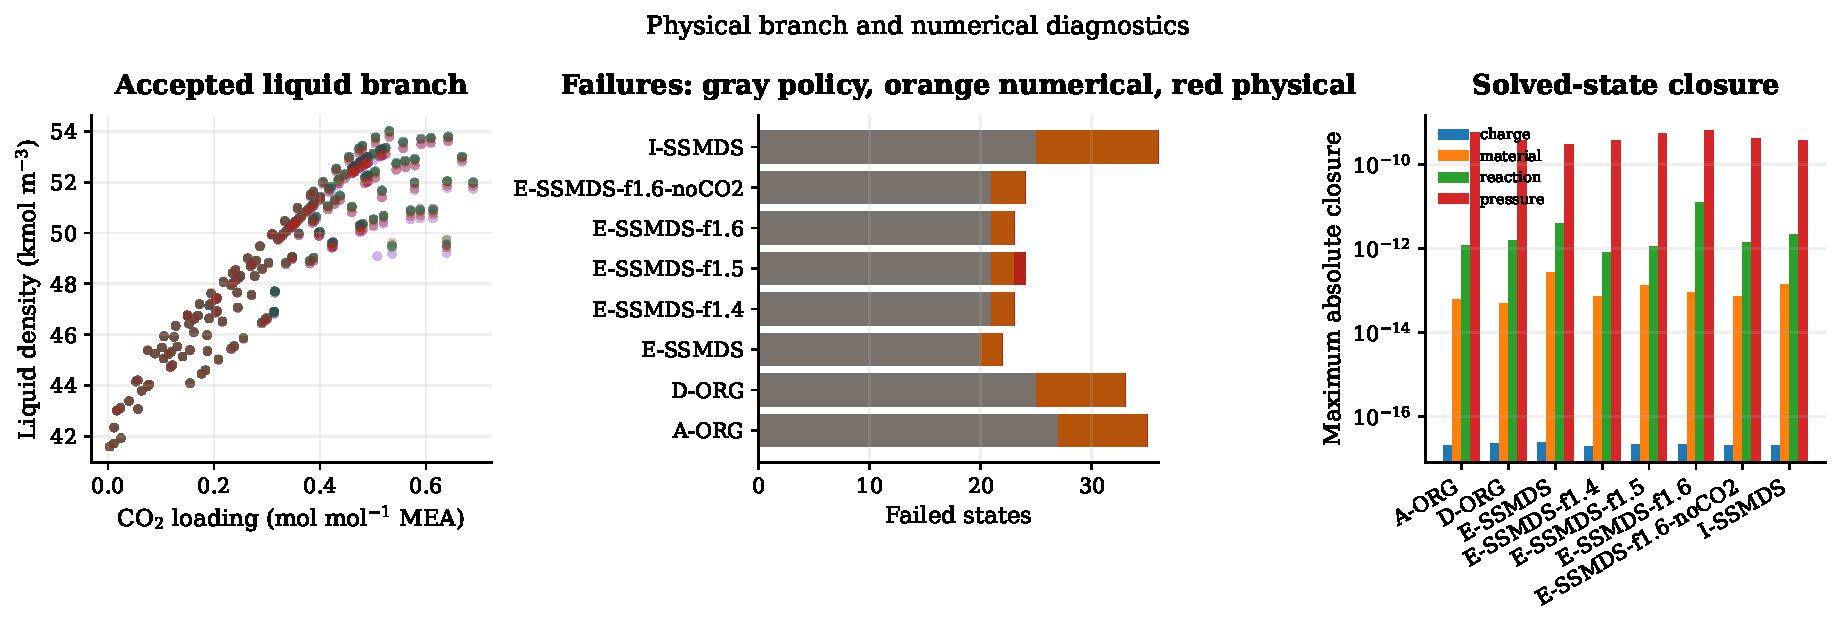
\includegraphics[width=\textwidth]{figures/born_permittivity/output/born-permittivity-diagnostics.pdf}
\caption{Accepted liquid density, preserved failure classes, and maximum
charge, material, reaction-affinity, and pressure closure for every promoted
configuration.}
\label{fig:born-permittivity-diagnostics}
\end{figure}

At the common \SI{40}{\celsius}, loading 0.389 state, A-original has
$(a^{\mathrm{Born}},a^{\mathrm{DH}},a^{\mathrm{res}})/(RT)=
(-13.8158,-0.0577,-22.4172)$; E--SSM+DS with $f_{\mathrm{MEA}}=1.6$ gives
$(-12.7242,-0.0989,-21.3758)$. The separated axes in
Figure~\ref{fig:born-permittivity-contributions} expose the otherwise hidden
Debye--H\"uckel change.

\begin{figure}[H]
\centering
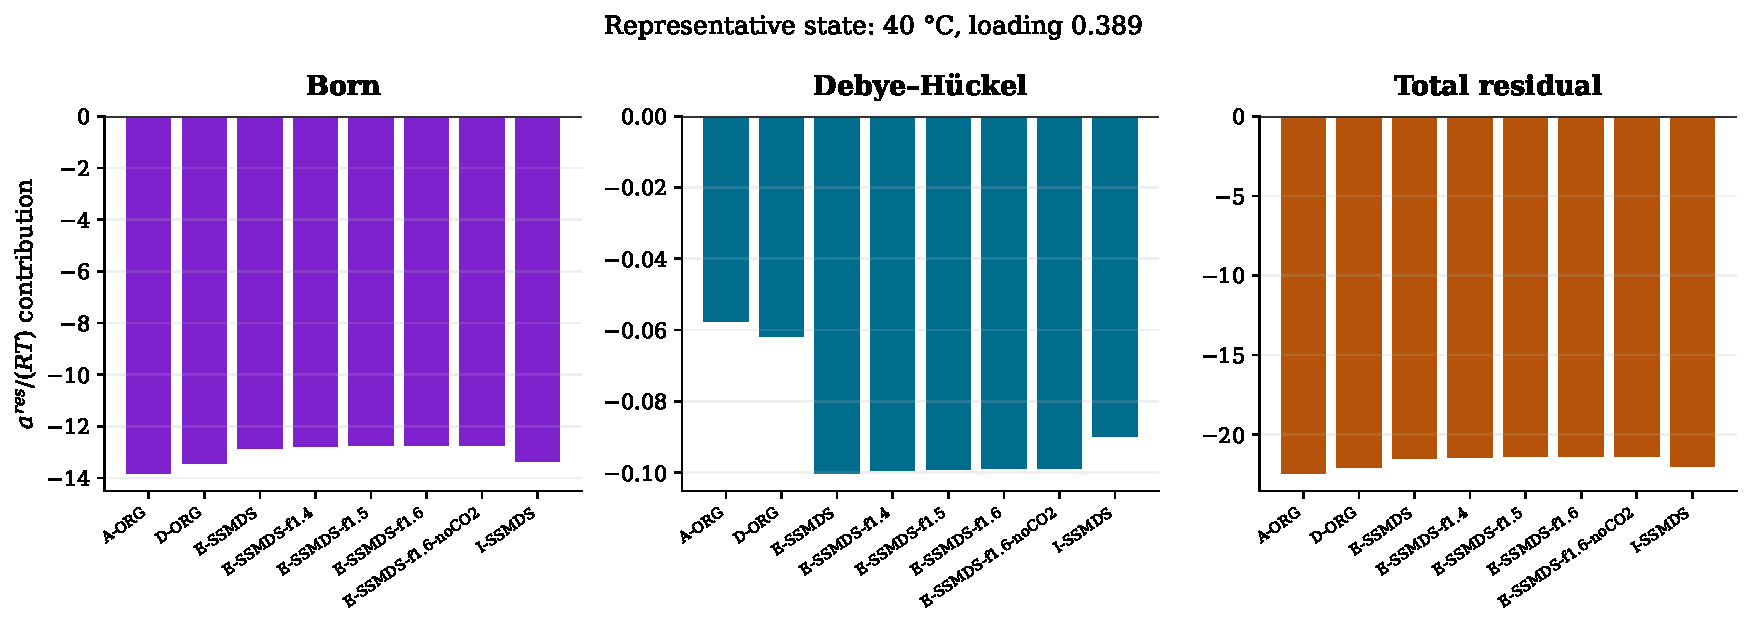
\includegraphics[width=\textwidth]{figures/born_permittivity/output/born-permittivity-contributions.pdf}
\caption{Born, Debye--H\"uckel, and total residual Helmholtz contributions at
one common representative state. Each panel has its own ordinate scale.}
\label{fig:born-permittivity-contributions}
\end{figure}

The retained dielectric folder contains no admitted static-permittivity data
for loaded aqueous MEA. The plotted Figiel relation is therefore a
literature-form crossover evaluated at this study's solved compositions, not
independent MEA validation. Within that limit, E predicts 26.54--60.19,
the Zuber analog/fallback suppression screen predicts 30.36--62.15, D predicts 44.00--70.80, and
A predicts 45.32--79.29 across successful states. Coupled molecular-
\ce{CO2} exclusion from both $f_{\mathrm{mix}}$ and the neutral dielectric
pool changes the universal-1.6 pressure log RMSE from 0.389898
to 0.387514, changes species log RMSE by less than $2\times10^{-7}$, and
has negligible effect on the present common-observation residuals.

\textbf{Current interpretation:} populated unique Born diameters and non-unit
neutral solvation factors activate SSM+DS. With the unadjusted R5 correlation,
that formulation worsens pressure. A bounded R5 movement nearly recovers the
original-Born pressure result and improves speciation, so the discrepancy is a
coupled reaction/electrostatic calibration problem rather than evidence for
turning SSM+DS off. Solvent-only mixing with SSM+DS and
R5 $a_K=2597.91$ K is the selected active configuration; nonlinear suppression with R5
$a_K+80$ K is the coverage and pressure-bias leader. Neither settles the
permittivity model without loaded-MEA dielectric observations and a consistent
Born-diameter/R5 fit. Explicit \ce{CO2} exclusion remains immaterial at the
present compositions.

\section{Current conclusions and next experiments}
\label{sec:next-experiments}

The selected physical structure includes reciprocal induced
\ce{CO2}-\ce{H2O} association and excludes \ce{CO2} self-association. The
active foundation uses corrected R1--R3, solvent-only mass-fraction dielectric
mixing, automatically activated SSM+DS,
and $k_{\ce{CO2},\mathrm{MEA}}=0$. The following
steps provide the shortest discriminating path. Items below are proposed work,
not retained results.

\begin{enumerate}
\item Preserve the certified loading/temperature continuation replay that
recovers all 161 pressure observations without changing parameters or
tolerances. Reduce the remaining three optional speciation display-grid
failures with the same branch-preserving method, and use those cases as
acceptance evidence for the upstream unified pressure--equilibrium KKT owner.
\item Complete the coupled bubble-pressure ablation with the active
parameter file: nine versus six liquid species, crossed with ePC-SAFT versus
ideal vapor. The retained comparison has already established the exact
six-species reaction projection, ideal-liquid behavior, fixed-$T,P$ liquid
behavior, and the failure of the neutral apparent-flash shortcut. Report state
evaluability, pressure and species metrics, charge/balance closure, and changes
by pressure range and temperature.
\item Freeze calibration and held-out source/temperature partitions, then
replay the sensitivity screen with the active parameter packet. Limit the
first pass to R4/R5, the bicarbonate and carbonate Born diameters, the three
Class~2 nonzero water--trace-ion corrections, and the seven named Class~2 zero
pairs. Do not run a broad fit until the recovered-state sensitivities show
which coordinates are identifiable from both pressure and speciation.
\item Seek simpler identifying evidence for the weak blocks: protonated-MEA
salt and bicarbonate activity, osmotic, density, or solvation data. Also admit
independent physical-solubility evidence before expanding the molecular model.
Jiru et al. measure physical \ce{CO2} solubility in MEA--water by the
\ce{N2O} analogy over 298.15--323.15 K \cite{Jiru2012}; Hartono et al. report
\ce{N2O} solubility in unloaded and loaded MEA \cite{Hartono2014}. Wong et al.
directly measure dissolved molecular \ce{CO2} and Henry behavior
\cite{wongSituMeasurementPhysical2016}, but every retained row contains
0.517 mol kg$^{-1}$ \ce{NaClO4}, which the nine-species model omits; use those
rows as an external challenge unless the salt is represented explicitly.
\item Use the completed 113-row direct total-enthalpy replay to identify the
smallest reaction-temperature correction supported simultaneously by pressure,
speciation, and calorimetry. Keep the 66 Kim--Svendsen 40/80~\si{\celsius}
rows as calibration, the 20 rows at \SI{120}{\celsius} as a temperature
holdout, and the 27 Kim 2014 rows as model-selection comparison evidence.
Before fitting, test the declared zero-vapor/ideal-feed reconstruction and the
first-row loading assumption. Do not copy the eNRTL block weight or numerical
reaction values.
\item Acquire or digitize independent static-permittivity observations for
loaded aqueous MEA. The completed fixed-parameter comparison cannot select
between the A and E dielectric responses from pressure and speciation alone,
and the Figiel relation is not an independent MEA measurement. Keep
solvent-only mass-fraction mixing as the active dielectric rule until that
evidence exists.
\item Continue Figiel's staged identification instead of fitting every radius
and solvent factor at once. Keep the
literature-anchored water factor at 1.5, omit molecular \ce{CO2} from the
solvent pool because its retained crossover was immaterial, and profile
$f_{\mathrm{solv},\mathrm{MEA}}$ jointly with each uncertain ion Born diameter
(with the two trace-carbonate diameters also tested as a pair). Every grid
member must use the same pressure and speciation rows. Promote only coordinates
whose pressure and species sensitivities are both non-flat and not mutually
compensating; then perform one bounded joint iteration and a held-out replay.
This is the shortest MEA analogue of Figiel's diameter--factor--$k_{ij}$ fitting
sequence and directly tests practical identifiability.
\item Only after these identifying experiments, run a bounded joint
optimization over the supported coordinates. With R1--R5, the ion block, and independently accepted
$k_{\ce{CO2},\ce{H2O}}$ fixed, compare only physical dissolved-\ce{CO2}
alternatives that the new data can distinguish: a \ce{CO2}--MEA association
edge, a physically identified solvation/activity contribution, and any richer
binary correction justified by the temperature and composition coverage. Do
not combine coordinates that the admitted observations cannot identify.
\item Require simultaneous comparative improvement in pressure, speciation,
and convergence coverage, followed by held-out temperatures and sources before
issuing an immutable packet. No unapproved numerical threshold is an
acceptance gate.
\end{enumerate}

\textbf{unknown:} whether ideal vapor, reduced chemistry, or neither materially
changes the coupled bubble-pressure residual has not been tested with the
active bundle.

Replace the current numerical foundation in place when a better MEA-owned
regression or validation result passes the stated comparison gates. Every
replacement must bind the Engine wheel and hash, parameter identities and
evidence status, admitted rows and hashes, optimizer diagnostics, validation
summaries, and the transfer decision. This PDF is the live calculation and
interpretation record for the active bundle, including the reported fit
statistics and state counts.

\subsection{Independent review record}

An independent read-only review on 2 September 2026 assessed commit
\nolinkurl{fb6f948}. It verified the 161-pressure plus 44-speciation scope,
the coupled \ce{CO2}-pool exclusion, normalized $f_{\mathrm{mix}}$, separate
source hashes, Rules B/C derivative checks, preserved failures, recomputed
summary metrics, and the synchronized 27-page render. The verdict was
\emph{Review Pass}: no material scientific, numerical, provenance, or layout
finding remained. The approved use is fixed-parameter model-structure
selection and failure characterization. It does not promote a new active
bundle, resolve the separate 319-row admission decisions, or supply missing
independent loaded-MEA static-permittivity observations.

\section{Provenance}

The base numerical reconstruction uses the PR \#134 file:\par\vspace{2pt}
\path{validation/campaigns/2026-mea-parameter-estimation/analysis/joint-fit/parameters.json}
\par\vspace{2pt}at commit
\nolinkurl{38e91823b6d4f26c1d549f07aaef24a089d8e16d}.
The selected live mapping is:\par\vspace{2pt}
\path{results/selected-current-best-parameters.json}
\par\vspace{2pt}Its SHA-256 is the parameter identity reported in Section 2.
The comparison result records both the base and selected fingerprints.

\begin{tabularx}{\textwidth}{@{}p{0.31\textwidth}Y@{}}
\toprule
Source & Role \\
\midrule
\href{https://github.com/tannerpolley/ePC-SAFT/issues/80}{ePC-SAFT Issue \#80} & Upstream full regression and immutable-packet campaign. \\
\href{https://github.com/tannerpolley/ePC-SAFT/issues/119}{ePC-SAFT Issue \#119} & Bounded refinement scope and current foundation reconciliation. \\
\href{https://github.com/tannerpolley/ePC-SAFT/pull/134}{ePC-SAFT PR \#134} & Closed, unmerged blocker-evidence change. It produced no parameter bundle; this notebook reconstructs only its frozen foundation vector. \\
Local component source audit & \path{docs/ePC-SAFT/full-component-parameter-source-audit.md}; species-level lineage and evidence gaps. \\
Local model-hierarchy review & \path{docs/ePC-SAFT/amine-epcsaft-model-hierarchy-literature-review.md}; selected nine-species structure and induced-association decision. \\
Retained parameter evidence & \path{analyses/reactive_epcsaft_parameter_evidence/}; supported-negative and diagnostic evidence. \\
Retained local-speciation fit & Git commit \texttt{897bb6e}; the May 2026 8-state/22-residual principal-ion fit retained as Class~3 evidence awaiting promotion checks. \\
Reaction exporter defect & \path{validation/campaigns/2026-mea-parameter-estimation/scripts/build_fit_input.py} at Engine commit \nolinkurl{38e91823b6d4f26c1d549f07aaef24a089d8e16d}. \\
Corrected start comparison & \path{results/parameter-start-comparison.csv}; full corrected-foundation and B\"ottinger-R4 comparison statistics. \\
Bounded sensitivity screen & \path{results/parameter-sensitivity-screen.csv}; common-row \ce{CO2}--MEA and \ce{CO2}--water perturbation results used in Section~\ref{sec:start-decision}. \\
Quick direct endpoint screen & \path{results/quick-endpoint-perturbation-screen.csv} and its JSON receipt; full reactive bubble-point endpoints and the bounded SciPy reaction-root spot check. \\
Best-in-slot campaign & \path{results/best-in-slot-campaign/}; centered sensitivity, R4 pivot--slope grids, full validations, boundary diagnostics, exact receipts, and the selected candidate's row-level Engine evaluations. \\
Born--permittivity structure study & \path{results/born-permittivity-study/}; exact sparse and complete state/target tables, failure characterization, grouped statistics, Engine parity and density-anchor timings, deterministic formulation construction, and hashes. Figures~\ref{fig:born-permittivity-overview}--\ref{fig:born-permittivity-contributions} read these retained values without rerunning the Engine. \\
Current Engine wheel & \path{data/input/engine/epcsaft-0.2.0.dev0-cp313-cp313-linux_x86_64.whl}; Engine commit \nolinkurl{8438ce5f94a547189c91c4ec180a7782d60879d6} and wheel SHA-256 \nolinkurl{40fba7cfb9c8414152f3e49636c49ae2e3f7099e30040d54d464ccb38355f805}. \\
Selected live mapping & \path{results/selected-current-best-parameters.json}; solvent-only mass-fraction mixing, automatic SSM+DS activation, the selected Class 3 R4--\ce{CO2} fit, and R5 $a_K=2597.91$ K. \\
Trace-species abundance & \path{figures/speciation/output/speciation-model.csv}; retained 44-state calculated values summarized in Section~\ref{sec:pressure-identifiability}. \\
Current IDAES comparison & Official public \href{https://github.com/IDAES/idaes-pse/blob/main/idaes/models_extra/column_models/properties/MEA_solvent.py}{MEA solvent} and \href{https://github.com/IDAES/idaes-pse/blob/main/idaes/models_extra/column_models/properties/MEA_vapor.py}{MEA vapor} property files; used only to define the proposed structural ablation. \\
Matched species comparison & \path{../enrtl_six_species_ideal_comparison/notebook.qmd} and \path{../enrtl_six_species_ideal_comparison/notebook.pdf}; exact ideal projection, fixed-$T,P$ Engine/SciPy comparison, corrected apparent-pressure diagnostic, parameter inventory, sensitivity survey, UQ checkpoints, and figures. \\
\bottomrule
\end{tabularx}

\appendix
\clearpage
\section{Additional-temperature speciation replays}
\label{sec:additional-speciation}

The following panels apply the same species selection, source encoding,
reported-zero omission, split-axis rule, parameter bundle, and pinned Engine
route as Figure~1. They are supplementary temperature views rather than
additional fits. At \SI{40}{\celsius}, 74 positive plotted values cover 21
states and observed loading 0.11--0.99; at \SI{60}{\celsius}, 21 values cover
eight states and observed loading 0.131--0.766; at \SI{80}{\celsius}, 14 values
cover six states and observed loading 0.064--0.51. Every model grid continues
to loading 1.0, and all 46 states evaluated at each temperature. Dashed lines
connect those direct calculations.

\begin{center}
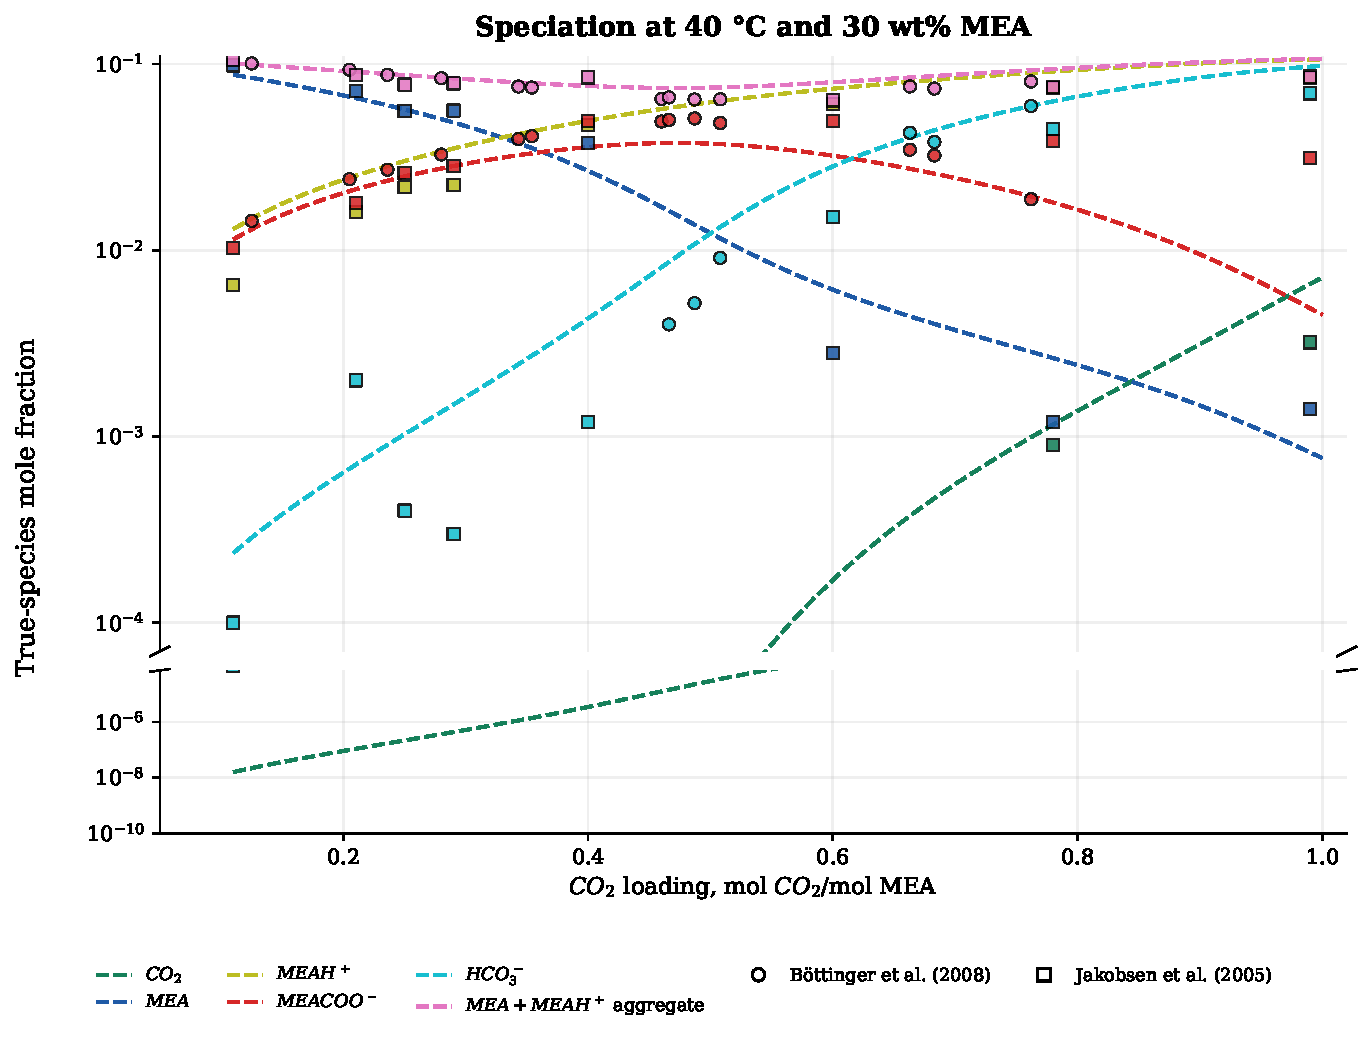
\includegraphics[width=\textwidth]{figures/speciation/output/speciation-diagnostic-replay-40C.pdf}

\small\textbf{Appendix Figure A1.} Principal-species replay at
\SI{40}{\celsius} and 30 wt\% MEA. Symbols retain every displayed B\"ottinger
and Jakobsen observation; dashed lines are direct Engine calculations.
\end{center}

\clearpage
\begin{center}
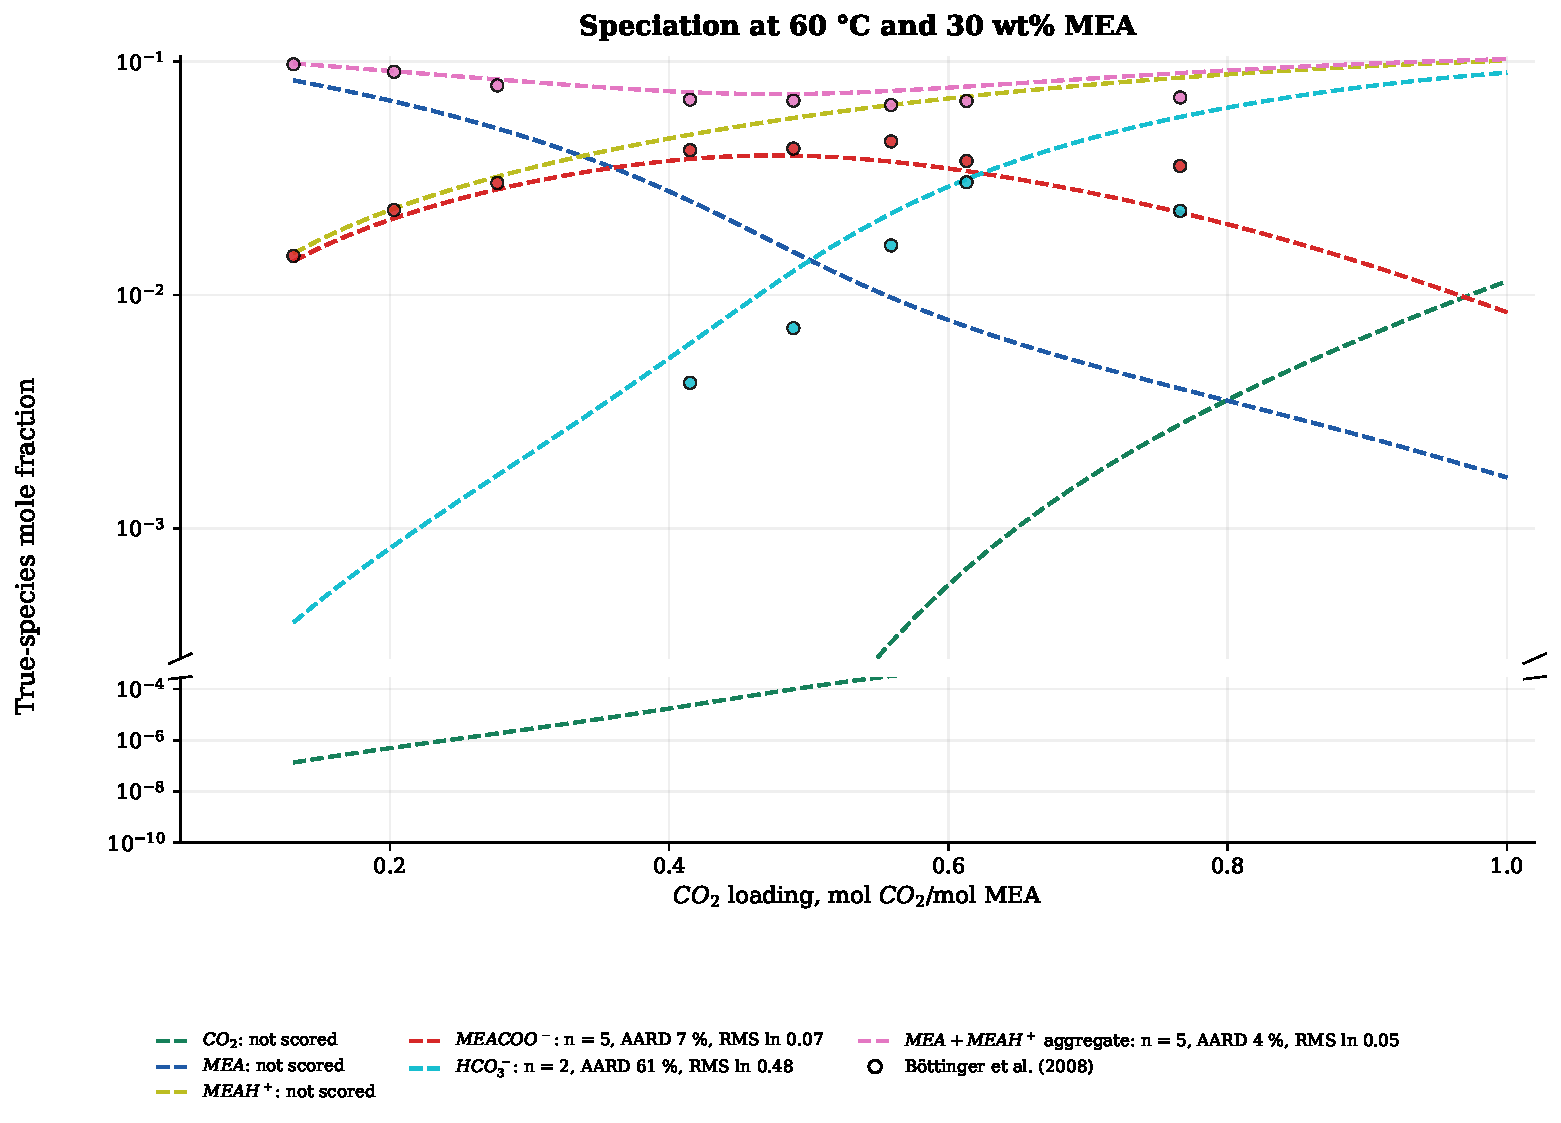
\includegraphics[width=\textwidth]{figures/speciation/output/speciation-diagnostic-replay-60C.pdf}

\small\textbf{Appendix Figure A2.} Principal-species replay at
\SI{60}{\celsius} and 30 wt\% MEA. Symbols retain every displayed B\"ottinger
observation; dashed lines are direct Engine calculations.
\end{center}

\clearpage
\begin{center}
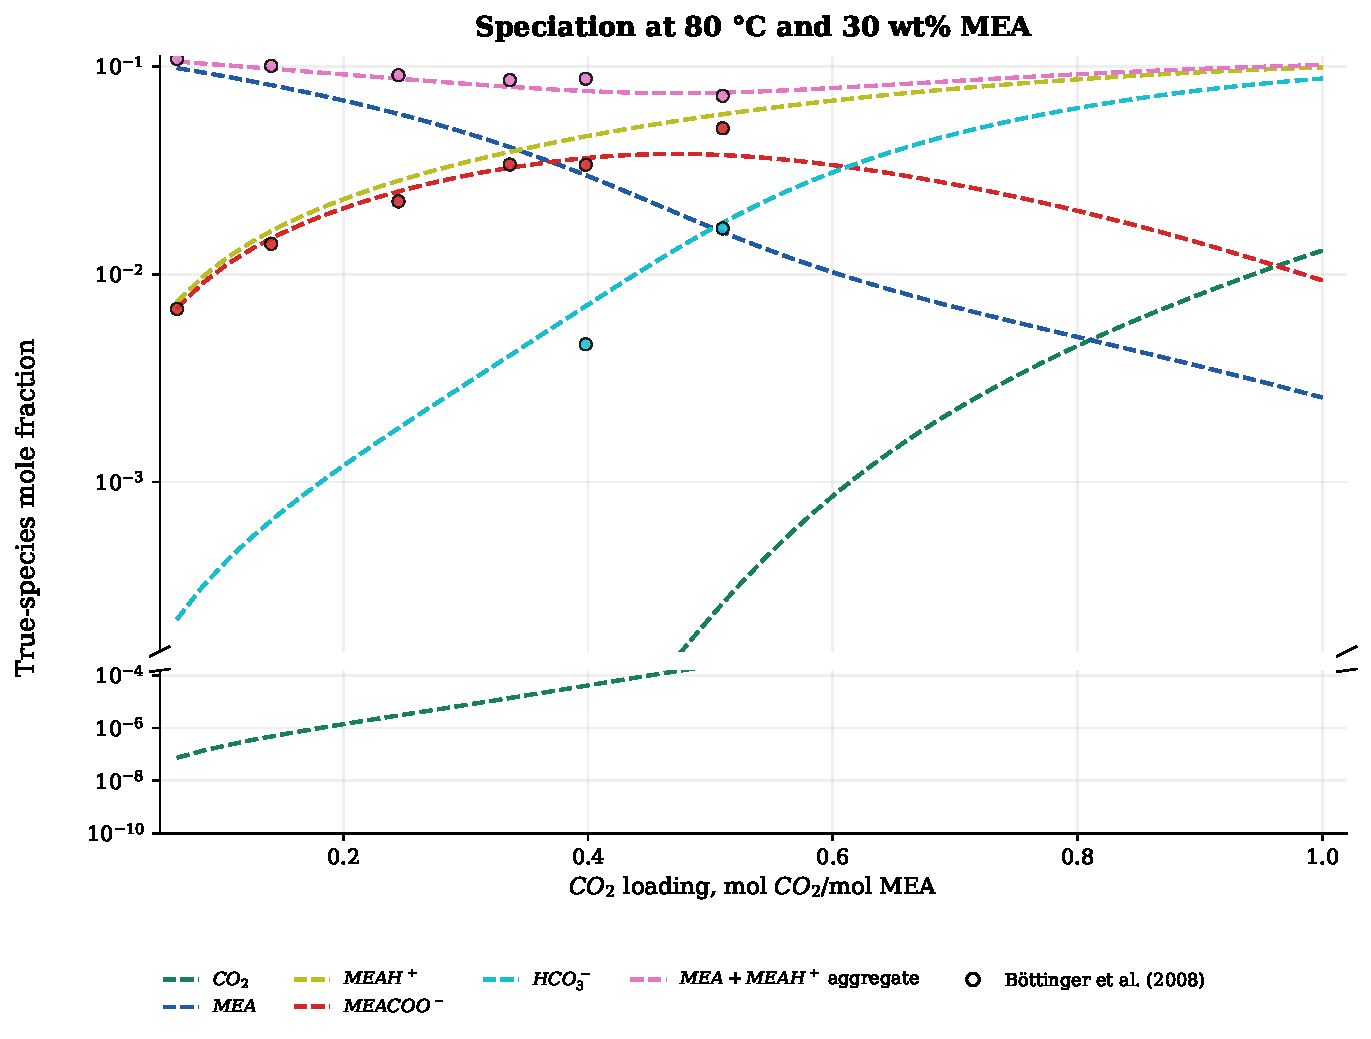
\includegraphics[width=\textwidth]{figures/speciation/output/speciation-diagnostic-replay-80C.pdf}

\small\textbf{Appendix Figure A3.} Principal-species replay at
\SI{80}{\celsius} and 30 wt\% MEA. Symbols retain every displayed B\"ottinger
observation; dashed lines are direct Engine calculations.
\end{center}

\begingroup
\setlength{\emergencystretch}{2em}
\printbibliography[title={References}]
\endgroup

\end{document}
